% ---------------------------------------------------------------------------
% PLOS ONE submission template.
% Preamble follows the official PLOS LaTeX template (PLOS_LaTeX_Template.tex).
% Compiles on Overleaf. For final submission, replace the figure PNGs with
% TIFF or EPS at >= 300 dpi and upload them as separate files, and switch the
% bibliography to plos2015.bst.
% ---------------------------------------------------------------------------
\documentclass[10pt,letterpaper]{article}
\usepackage[top=0.85in,left=2.75in,footskip=0.75in,marginparwidth=2in]{geometry}

\usepackage{amsmath,amssymb}
\usepackage{changepage}
\usepackage[utf8]{inputenc}
\usepackage{textcomp,marvosym}
\usepackage{cite}
\usepackage{nameref,hyperref}
\usepackage[right]{lineno}
\usepackage{microtype}
\DisableLigatures[f]{encoding = *, family = * }

\usepackage[table]{xcolor}
\usepackage{array}
\usepackage{booktabs}
\usepackage{graphicx}
\usepackage{fancyhdr}
\pagestyle{myheadings}

% Text layout, per PLOS template
\raggedright
\setlength{\parindent}{0.5cm}
\textwidth 5.25in
\textheight 8.75in

% Bold "Fig N." and separate from caption with a period
\usepackage[aboveskip=1pt,labelfont=bf,labelsep=period,
            justification=raggedright,singlelinecheck=off]{caption}
\renewcommand{\figurename}{Fig}

% Remove brackets from reference numbering
\makeatletter
\renewcommand{\@biblabel}[1]{\quad#1.}
\makeatother

% Short running head for the derived plain-article version.
% RUNNINGHEAD: Street slope and property crime

% Leave date blank
\date{}

% PLOS does not want figures embedded in the manuscript PDF -- they are uploaded
% as separate TIFF files (outputs/plos_figs/Fig1.tif ...). Keep this false for
% submission; flip it to \embedfigstrue to compile a reading copy with the
% images in place.
\newif\ifembedfigs
\embedfigsfalse

\begin{document}
\vspace*{0.2in}

\begin{flushleft}
{\Large
\textbf\newline{Street slope and reported property crime in nine United States
cities: terrain measurement, target exposure, and tests of candidate mechanisms}
}
\newline
\\
Walker Tracy\textsuperscript{1*}
\\
\bigskip
\textbf{1} University of Utah, Salt Lake City, Utah, United States of America
\\
\bigskip
* walkeratracy@gmail.com
\end{flushleft}

% ---------------------------------------------------------------------------
\section*{Abstract}

Steeper streets carry less crime. Haberman and Kelsay established this for robbery
in Cincinnati, estimating roughly 4.5\% fewer robberies per one percent increase in
street block slope, and they closed their paper by naming three possible reasons for
it: steep blocks raise the physical costs of offending, they are difficult to escape
from, and they carry fewer people. They did not test between those three
explanations. That is the gap this paper is written to fill. Using incident level
property crime from nine American cities, lidar elevation from the United States
Geological Survey, building footprint exposure denominators, and census block group
fixed effects, I report four findings. First, the negative slope association
generalizes from robbery to property crime. All nine cities show significantly less
recorded property crime on steeper streets, and among the four cities with the most
measurable gradient a random effects pool gives $-6.89\%$ per degree of slope
(95\% CI $[-9.51, -4.21]$). The heterogeneity is severe: $I^2 = 0.75$, and the
prediction interval for a new city runs from $-13.7\%$ to $+0.5\%$, so this should
not be read as a transportable coefficient. Rather than split the sample at a
threshold chosen after seeing the terrain data, I model the city effect as a
continuous function of how much gradient a city has to measure; that moderator
accounts for 59\% of the between city variance. Second, the association is not
explained by the cost of carrying loot. I use a control the literature has not
used, which is vandalism and arson: property crimes in which nothing is removed.
These hold the cost of approach roughly constant while setting the cost of removal
to zero, so a loaded haul account requires them to be markedly less affected. They
are not, and an equivalence test rejects a difference as large as half the headline
effect. The result survives dropping arson and reweighting the two offense groups
to a common hour by day of week distribution. Third, street network structure
absorbs about a quarter of the association, which is a substantial share and not a
failed explanation. Fourth, the strongest available objection, that steep cells
simply hold fewer targets, does not account for it in San Francisco, where
replacing the housing denominator with on street parking capacity and front doors
makes the estimate more negative rather than less. An attempt to extend that test
nationally using building footprint counts is largely uninformative: the model
fails to converge in five of nine cities, and in the four where it does the
denominator changes the estimate by less than 1.5 percentage points in either
direction. None of the mechanisms I could test accounts for the association, and
I decline to supply one I cannot test. What
I report is a robust conditional association, not a demonstration that gradient
deters offenders.

% ---------------------------------------------------------------------------
\linenumbers

\section*{Introduction}

\subsection*{Motivation and objectives}

Environmental criminology holds that offenders are effort minimizing. They offend
inside the space they already know, close to the places they already go, and they
travel no further than they need to. This is the principle of least effort, and it
sits underneath crime pattern theory \cite{brantingham1993} and routine activity
theory \cite{cohen1979}, and underneath distance decay in the journey to crime,
which is one of the most reliable empirical regularities the field has.

Terrain is an obvious place to apply that idea. If horizontal distance costs effort,
then gradient should cost more of it. A literature has looked, and it does not agree
with itself. Breetzke found that burglary in Tshwane fell with altitude, but that
slope had no effect at all, which is strange if the mechanism is energetic, since
steepness is exactly where the energy cost lives \cite{breetzke2012}. Haberman and
Kelsay found the opposite in Cincinnati: street block slope predicted fewer
robberies, at roughly 4.5\% per one percent of grade \cite{haberman2021}. Kim and Wo
found that in San Francisco all of their topographic measures mattered, with
elevation \emph{differences} in the surrounding quarter mile the strongest of them,
but a segment's own elevation and slope also significant \cite{kimwo2023}. Two
recent bicycle theft studies split the same way: Christiansen and Pires report a
negative street slope association in San Francisco \cite{bikesf2026}, while
Christiansen's Toronto study reports negative elevation and hilliness effects with
slope itself not significant \cite{biketoronto2026}.

The economics literature reached the terrain question earlier and from a different
direction. Ye and Becker analyzed elevation gradients across seventeen American
cities and documented that high income households prefer both altitude and
unevenness, producing income stratification along the vertical dimension of a city
\cite{yebecker2018}; they extend the argument to neighborhood sorting in later work
\cite{yebecker2024}. That literature matters here for two reasons. It means a
multi-city American topography study is not itself novel, and it means the
confounding problem this paper has to solve is a documented empirical regularity
rather than a hypothetical one.

For example, imagine two houses on the same block, one at the bottom of a hill and
one at the top. The literature above says the house at the top is safer. It does not
say why, and the reason matters enormously, because the three available reasons imply
completely different things about what to do with the finding.

Haberman and Kelsay stated the open question precisely. Steeper blocks, they
concluded, may have fewer robberies because they make the physical costs of
committing robberies too high, because they are too difficult to escape from, and/or
because they provide fewer opportunities owing to relatively lower usage. That is
three mechanisms, one observed sign, and no test between them:

\begin{itemize}
\item \textbf{M1, effort.} Climbing and hauling cost energy, so offenders substitute
toward easier targets.
\item \textbf{M2, exposure and risk.} Steep streets carry less through traffic, offer
fewer escape routes, and are overlooked from below. Fewer offenders pass by at all,
and the ones who do are more exposed.
\item \textbf{M3, confounded affluence.} Terrain is capitalized into land value.
Hills are wealthy, and wealth predicts guardianship and target hardening.
\end{itemize}

My objective in this research was to build a design in which those three mechanisms
make different predictions, and then to run it. Specifically I set out to: (i) test
whether the slope finding generalizes from robbery in one city to property crime
across many; (ii) separate the cost of \emph{reaching} a target from the cost of
\emph{removing} something from it; (iii) measure the street network channel rather
than merely naming it; (iv) test whether the whole thing is a denominator artifact;
and (v) report what survives, honestly, including when nothing does.

One thing I want to be clear about at the outset, because it governs how every
result below should be read. This is an observational design. Block group fixed
effects remove everything that is constant across a block group, which is a great
deal, but they do not make slope as good as randomly assigned inside one. A steep
street and a flat street in the same block group can still differ in building form,
frontage, lighting, parking regulation, through traffic and willingness to report,
and nothing in this design separates those from gradient. What I can establish is
that a conditional association exists, that it is large, and that several specific
explanations for it do not work. I cannot establish that gradient deters anybody.
The literature that can speak to offender decisions directly does so with cleared
offenses and discrete choice models over the alternatives an offender did not pick
\cite{frith2017,johnsonsummers2015,clare2009}, and I say more in the Discussion
about why that is the design this question eventually needs.

\subsection*{The no-loot control}

The central idea of this paper is simple enough to state in a sentence. Not all
property crime involves carrying anything away.

Vandalism and arson are property crimes in which the offender removes nothing.
Reaching the target costs a vandal roughly what it costs a burglar. Leaving costs the
vandal nothing extra.

That makes them a negative control for the removal channel specifically. Under M1,
the terrain coefficient for no-loot crime has to be markedly closer to zero than the
coefficient for theft, because half of the energetic penalty, which is the loaded
return trip, is absent by construction. Under M2 and M3 the two should look the same,
because through traffic, sightlines, escape routes and affluence do not care whether
anything was taken.

I want to be careful about how much this comparison can carry, because it is the
paper's most original move and it is easy to overstate. It is not a placebo in the
strict sense, and I no longer describe it as one. Vandalism, arson and theft differ
in far more than the weight of what leaves the scene: in offender age, motive,
planning, time of day, co-offending, tool use, and in how reliably a victim reports
them. A null difference therefore falsifies one specific quantitative implication,
that the slope coefficient is driven mainly by the metabolic cost of hauling stolen
goods along a gradient. It does not falsify effort in general. The cost of walking
up to a target, the offender's perception of that cost, search costs and escape risk
are all untouched by this test, and I take some care later not to let the conclusion
drift into them.

Two of the obvious objections to the comparison can be answered directly, and I
answer both in the Results. Arson is not vandalism and involves preparation and
acute escape risk, so I separate them and re-run the test on vandalism alone.
Vandalism concentrates at night and theft does not, so I reweight the two groups to
a common hour by day of week distribution and re-run it again. The comparison is
internal in either version: the same city, the same block groups, the same
covariates and the same terrain measure, and it requires no data beyond a crime type
split.

\subsection*{Paper structure}

The rest of this paper is organized as follows. The Materials and methods section
describes the crime data, the terrain measures, the exposure denominators, the
estimator, and the inclusion rule. The Results section reports the slope association
and its heterogeneity, including a random effects synthesis and a moderator model
that replaces the threshold I originally used, then works through the mechanism
tests in order, then reports the robustness analyses and the measurement findings
that bear on how this literature should be conducted. The Discussion returns to the
three mechanisms Haberman and Kelsay named and explains what this design can and
cannot say about each. A short Conclusion, statements on ethics and on the software
and AI tooling behind the paper, a list of further research ideas, and recognitions
follow.

% ---------------------------------------------------------------------------
\section*{Materials and methods}

\subsection*{Crime data}

I use incident level records with point coordinates from municipal open data portals,
covering 2018 onward (Baltimore from 2022, Charlotte from November 2019, and
Pittsburgh through November 2023, which is where that city's incident level
publishing stops). Offense descriptions are mapped onto an ordered loot mass ladder,
running from pocketable theft at roughly 0.3~kg up to catalytic converter removal and
similar at 25~kg, plus two classes that sit outside the ladder deliberately:
\texttt{MVT} for motor vehicle theft, where the goods drive themselves away, and
\texttt{NO\_LOOT} for vandalism, criminal damage and arson. The mapping was fixed
before any outcome analysis was run.

One methodological note belongs here rather than in a footnote, because it determined
which cities could be analyzed at all. Description fields are selected by \emph{rank}
rather than by the order they appear in the dataset. An offense description outranks
a weapon, premises, victim or case status field. Los Angeles was initially absent from
this study entirely because it lists \texttt{weapon\_desc}, \texttt{premis\_desc} and
\texttt{vict\_descent} ahead of \texttt{crm\_cd\_desc}, so a harvester taking the
first three description columns was feeding the classifier a weapon, a premise and a
victim's ethnicity while discarding the only field that named the offense.

\subsection*{Terrain measures}

Elevation comes from the United States Geological Survey 3D Elevation Program at
10~m resolution, bare earth, referenced to NAVD88, and held at uniform resolution
across every city so that a terrain measure means the same thing everywhere.

Slope is computed with Horn's method \cite{horn1981}. Relative height is computed as the Topographic
Position Index, which is a cell's elevation minus the mean elevation within a radius
$R$ \cite{weiss2001}, evaluated at $R \in \{50, 100, 250, 500, 1000, 2000\}$~m. The
neighbourhood means are computed by FFT convolution together with a matching
convolution of the validity mask, which is what makes coastlines behave: a cell on
the shore is compared against the land around it rather than against a pile of
implicit zeros.

\subsection*{Unit of analysis and exposure}

The primary unit is the 100~m grid cell, with street segments built from OpenStreetMap
for four cities as the confirmatory unit and the only one on which network measures
are defined. Segments are also the unit the micro-places literature is built on
\cite{weisburd2015}, which makes the results directly comparable to it.

Exposure is the denominator that turns counts into rates, and it is where this kind
of study most easily goes wrong. The conventional choice is to apportion census
housing units to analysis units by land area, which quietly assumes that development
is spread evenly inside a block group. In sprawling places it is not. I therefore
apportion housing units and population by \emph{residential building footprint area},
using Microsoft Building Footprints.

\subsection*{Estimator}

All models are Poisson pseudo-maximum-likelihood with a log exposure offset and
\emph{absorbed census block group fixed effects}, with standard errors clustered on
block group. The reason for Poisson is not that the counts are overdispersed, which
was how I put it in an earlier draft and is not the argument. It is that the
conditional mean is multiplicative and the outcome has many zeros, and that pseudo
maximum likelihood estimates such a mean consistently whether or not the variance is
Poisson, provided inference is made robust \cite{silva2006}. Absorbed fixed effects
rather than dummy variables because five hundred to twenty-five hundred dummies make
the iteratively reweighted least squares fitter diverge; the inner weighted
demeaning loop is the one used by \texttt{ppmlhdfe} \cite{correia2020}.

The implementation is my own, in Python 3.13 with NumPy 2.3 and pandas 3.0, and the
details matter enough to state. The inner loop runs to a coefficient tolerance of
$10^{-9}$ with a cap of sixty iterations. Standard errors come from a cluster robust
sandwich on the absorbed design with a $G/(G-1)$ finite sample correction. Because a
high dimensional sparse count model can fail to have a maximum likelihood at all
\cite{correia2020}, I report the diagnostics in the Results: every city converged,
in eight to eleven iterations, with no separated observations and no singleton block
groups.

The consequence for interpretation is that identification is always \emph{within
neighbourhood}. Every comparison is between cells in the same census block group, so
everything constant across that block group is differenced away: its demographics,
its zoning, its police beat, its reporting regime. In an earlier draft I described
this as comparing the top of a hill against the bottom of the same hill. That
overstates what the estimator does. It compares all cells inside a fixed effect
stratum conditional on the covariates; it does not construct matched hilltop and
hillfoot pairs, and it does not remove anything that varies \emph{within} a block
group and happens to correlate with slope.

\subsection*{The paired test}

The theft and no-loot coefficients are estimated on the same units with the same
covariates, so they are correlated, and comparing their confidence intervals for
overlap would be wrong in an unknown direction. I bootstrap the difference directly,
resampling whole block groups, which is the level the standard errors are clustered
at, and refitting both models inside every draw so that the correlation between the
two estimates is carried through automatically.

\subsection*{Inclusion}

Cities enter the panel on terrain and volume only, never on the outcome coefficient:
at least 20,000 classified property crime incidents, and at least one incident per
analysis unit so that the crime feed actually covers the geography assigned to it.
All nine cities meeting those rules are reported throughout.

An earlier version of this paper added a third rule, a within-city slope standard
deviation of at least 3$^\circ$, and reported the four qualifying cities as the
headline. That threshold was chosen after looking at the terrain data. I have
demoted it. The primary analysis now models the city effect as a continuous
function of how much gradient a city has to measure, which uses all nine cities and
treats terrain measurability as the continuous quantity it actually is. The
threshold split is retained below it as a sensitivity analysis, which is the rank
it deserves.

% ---------------------------------------------------------------------------
\section*{Results}

\subsection*{The slope effect generalizes, and it is heterogeneous}

Every one of the nine cities shows significantly less recorded property crime on
steeper streets. The per-degree magnitude, however, varies enormously, and it varies
systematically with how much gradient a city has for the elevation model to measure
(Table~\ref{tab:panel}, Fig~\ref{fig:gradient}).

\begin{table}[!ht]
\centering
\caption{{\bf Effect of one additional degree of street slope on property crime.}
Poisson pseudo-ML, log exposure offset, absorbed block group fixed effects, standard
errors clustered on block group.}
\label{tab:panel}
\begin{tabular}{lrrl}
\toprule
City & Slope SD & Per degree & 95\% CI \\
\midrule
Pittsburgh & 4.82$^\circ$ & $-9.32\%$ & $[-11.11, -7.49]$ \\
San Francisco & 4.54$^\circ$ & $-7.02\%$ & $[-8.94, -5.06]$ \\
Seattle & 4.10$^\circ$ & $-5.73\%$ & $[-6.96, -4.47]$ \\
Cincinnati & 3.36$^\circ$ & $-5.83\%$ & $[-7.38, -4.25]$ \\
\textbf{Random effects pool} & & $\mathbf{-6.89\%}$ & $\mathbf{[-9.51, -4.21]}$, $I^2 = 0.75$ \\
\midrule
Baltimore & 2.15$^\circ$ & $-7.74\%$ & $[-9.86, -5.57]$ \\
Kansas City & 1.98$^\circ$ & $-13.93\%$ & $[-16.74, -11.02]$ \\
Montgomery County MD & 1.96$^\circ$ & $-21.55\%$ & $[-24.05, -18.97]$ \\
Charlotte & 1.81$^\circ$ & $-18.64\%$ & $[-21.63, -15.53]$ \\
Chicago & 0.93$^\circ$ & $-19.76\%$ & $[-23.30, -16.18]$ \\
\textbf{Random effects pool} & & $\mathbf{-16.37\%}$ & $\mathbf{[-22.95, -9.24]}$, $I^2 = 0.94$ \\
\midrule
\textbf{All nine cities} & & $\mathbf{-12.23\%}$ & $\mathbf{[-17.06, -7.12]}$, $I^2 = 0.98$ \\
\bottomrule
\end{tabular}
\end{table}

\paragraph{How the pooling is done, and why the interval got wider.} An earlier
draft pooled these estimates by inverse variance and printed $I^2$ beside the
result. That is a fixed effect pool. It answers what the common effect is on the
assumption that a common effect exists, and its interval narrows as cities are
added even when the cities visibly disagree; reporting a high $I^2$ next to it does
not repair the interval, it only announces that the model producing the interval is
wrong. The pools above are random effects, with $\tau^2$ by REML and a
Hartung-Knapp adjustment, which refers the interval to a $t$ distribution and
accounts for having estimated $\tau^2$ from a handful of cities \cite{intHout2014}.
With four cities that adjustment is not cosmetic: for the higher gradient group it
widens the 95\% interval from $[-8.50, -5.26]$ to $[-9.51, -4.21]$.

Three numbers matter more than the pooled point estimate. Between-city variance is
$\tau^2 = 0.00023$ for the higher gradient group, against $0.00518$ across all nine.
$I^2$ is 0.75 for the higher gradient group, but its Q-profile interval
\cite{viechtbauer2007} runs from 0.19 to 0.98, which is the honest statement at
$k=4$: I can tell that heterogeneity is present and almost nothing about how much
\cite{higgins2002}. And the prediction interval, which is the quantity a reader
actually wants when asking whether this transports, runs from $-13.7\%$ to
$+0.5\%$. A tenth city with real gradient could plausibly show no association at
all. Nothing in this paper should be read as licensing a point estimate for a city
not in it.

Leaving out one city at a time, the higher gradient pool ranges from $-6.01\%$ to
$-7.36\%$, so no single city carries it. It is worth noting that dropping
Pittsburgh, the largest individual estimate, takes $I^2$ from 0.75 to 0.00 and
tightens the interval to $[-7.53, -4.47]$. Almost all of the detectable
heterogeneity in that group is Pittsburgh being more negative than the rest.

\paragraph{Comparison to the prior estimate.} Haberman and Kelsay report approximately
4.5\% fewer robberies per one percent increase in street block slope, with slope
measured as percent grade. One degree of angle is $\tan(1^\circ) = 1.746\%$ grade, so
under a log link their coefficient converts to $-7.72\%$ per degree, since
$\beta = \ln(0.955) \times 1.746 = -0.0804$. That sits inside the range I find for
property crime among the higher gradient cities, which runs from $-5.73\%$ to
$-9.32\%$, and it is close to my pooled $-6.89\%$. A different crime type, a different
city, a different decade and a different estimator landing in the same band is
meaningful external validation of the magnitude.

Two qualifications belong with that comparison. Their outcome is robberies per foot of
block length rather than per target at risk, so the estimands are not identical. And I
was not able to obtain the full text, because the journal is paywalled and the
repository copy returns an HTTP 403, so the effect size, the percent grade units and
the three proposed mechanisms are all taken from the published abstract and from
secondary summaries. The conversion above should be confirmed against the original
before publication, and I would rather flag that than present it as verified.

\paragraph{It is not a constant, and I want to be clear about that.} An earlier
version of this analysis ran on three cities, found $I^2 = 0.00$, and I was tempted to
report a constant. Adding Pittsburgh, which played no part in selecting either the
variable or the inclusion rule, moved heterogeneity to $I^2 = 0.75$ ($Q = 11.4$ on
3~df, $p = 0.010$). With three studies a $Q$ test has two degrees of freedom and
almost no power, so $I^2 = 0.00$ there meant "undetectable" rather than "absent"
\cite{higgins2002}. I report the pooled figure with its heterogeneity and its
prediction interval attached, and I caution against treating any single number here
as a transportable coefficient.

\paragraph{Terrain measurability as a continuous moderator, not a threshold.} The
version of this paper I wrote first cut the sample at a within-city slope standard
deviation of 3$^\circ$ and reported the four cities above it as the headline. The
substantive argument for that cut is real: below roughly 3$^\circ$ a bare earth
elevation model at 10 m is measuring crowned roadbeds, embankments, railway grades
and ravine edges, none of which are terrain and all of which track land use. But the
number 3 came from looking at the terrain data, and a threshold chosen that way is a
researcher degree of freedom whatever the story attached to it, particularly when it
sets the headline number.

So the primary analysis is now a random effects meta-regression of the city
coefficient on that city's slope standard deviation, centred at 3$^\circ$, using all
nine cities (Table~\ref{tab:metareg}, Fig~\ref{fig:gradient}). The moderator is
strongly related to the effect: each additional degree of within-city slope
variation moves the per-degree coefficient $+4.06\%$ ($p = 0.020$), that is, toward
zero. It accounts for 59\% of the between-city variance, dropping residual $\tau^2$
from $0.00518$ to $0.00211$. The fitted effect is $-18.5\%$ per degree at a slope SD
of 1$^\circ$, $-11.8\%$ at 3$^\circ$, and $-6.3\%$ at 4.5$^\circ$.

That is a stronger and more honest version of the original claim. It says the same
thing the threshold said, namely that estimates from cities with little measurable
gradient are systematically larger, but it says it without cutting anything, it uses
every city, and it can be checked against a continuous prediction rather than a
binary one.

\begin{table}[!ht]
\centering
\caption{{\bf Random effects meta-regression of the city slope coefficient on how
much gradient the city has.} Nine cities. The moderator is centred at 3$^\circ$, so
the intercept is the fitted effect at the threshold used in the earlier draft.
Knapp-Hartung adjusted, $t$ on 7 df.}
\label{tab:metareg}
\begin{tabular}{lrrrr}
\toprule
Term & Coefficient & \% per degree & 95\% CI (\%) & $p$ \\
\midrule
Intercept (at SD $=3^\circ$) & $-0.1251$ & $-11.76$ & $[-15.30, -8.07]$ & 0.0002 \\
Slope SD $-\,3^\circ$ & $+0.0398$ & $+4.06$ & $[+0.84, +7.38]$ & 0.0202 \\
\midrule
\multicolumn{5}{l}{Residual $\tau^2 = 0.00211$ vs $0.00518$ unconditional; $R^2 = 0.59$} \\
\bottomrule
\end{tabular}
\end{table}

\paragraph{The threshold split, retained as a sensitivity analysis.} Cutting at
3$^\circ$ gives $-6.89\%$ above and $-16.37\%$ below, and the lower gradient group
is far more heterogeneous ($I^2 = 0.94$ against $0.75$). Charlotte arrived out of
sample after the threshold was set, fell below it, and returned $-18.64\%$ per
degree, as predicted.

Baltimore is the exception. At 2.15$^\circ$ it sits below the threshold but returns
$-7.74\%$, which is inside the higher gradient band. I report this rather than
adjusting the threshold to exclude it. Under the continuous model Baltimore is
simply a city whose effect sits well above the fitted line, which is a more useful
way to describe it than as a rule violation: with $R^2 = 0.59$, 41\% of the
between-city variance is still unexplained, and Baltimore is where a good deal of it
lives.

\begin{figure}[!ht]
\centering
\ifembedfigs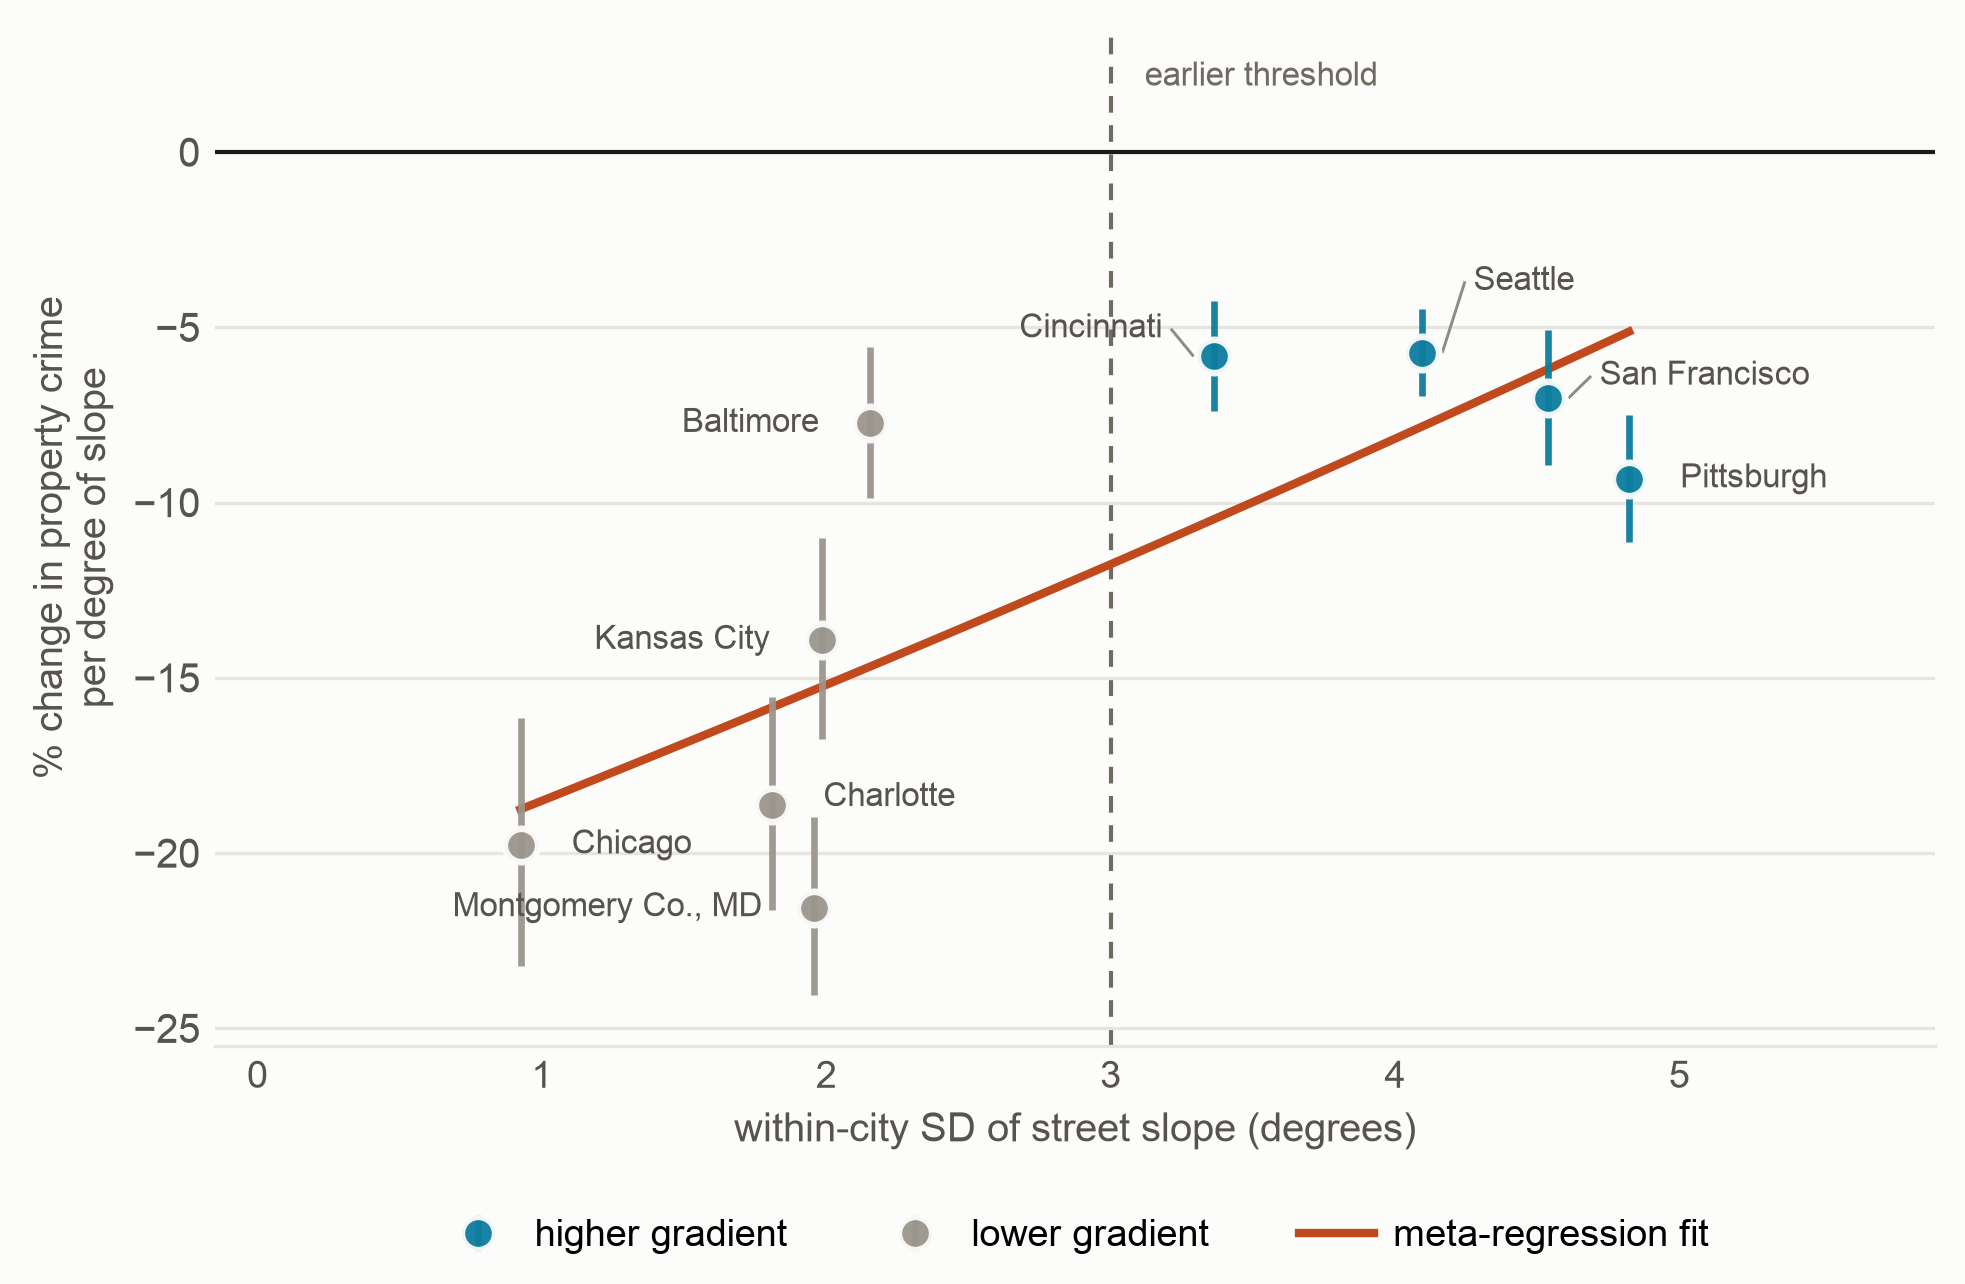
\includegraphics[width=\linewidth]{outputs/fig1_gradient_floor.png}\fi
\caption{{\bf Cities with less measurable gradient return systematically larger
per-degree estimates.} Each point is one city's estimated change in property crime
per additional degree of street slope, plotted against how much within-city slope
variation that city has. Vertical bars are 95\% confidence intervals. The line is
the random effects meta-regression fit of Table~\ref{tab:metareg}, which accounts
for 59\% of the between-city variance. The dashed marker at 3$^\circ$ is the
threshold used in an earlier draft, shown for reference only; it no longer defines
the sample. Baltimore is the city furthest above the fitted line and is discussed in
the text.}
\label{fig:gradient}
\end{figure}

\subsection*{Relative height is the unreliable measure}

Standardized within city, slope predicts less property crime in all nine cities, ranging
from $-15.8\%$ to $-37.9\%$ per standard deviation. Relative height, which is the
Topographic Position Index and the measure Kim and Wo emphasize, does not. It ranges from
$-10.7\%$ in Seattle to $+18.0\%$ in Charlotte and it changes sign in four of the nine
(Fig~\ref{fig:slopeheight}). In San Francisco it also depends on the unit of analysis, giving
$-9.2\%$ at 100~m cells and $+0.1\%$ at street segments, while slope is negative under
both. Where the two measures disagree, slope is the one that replicates.

\begin{figure}[!ht]
\centering
\ifembedfigs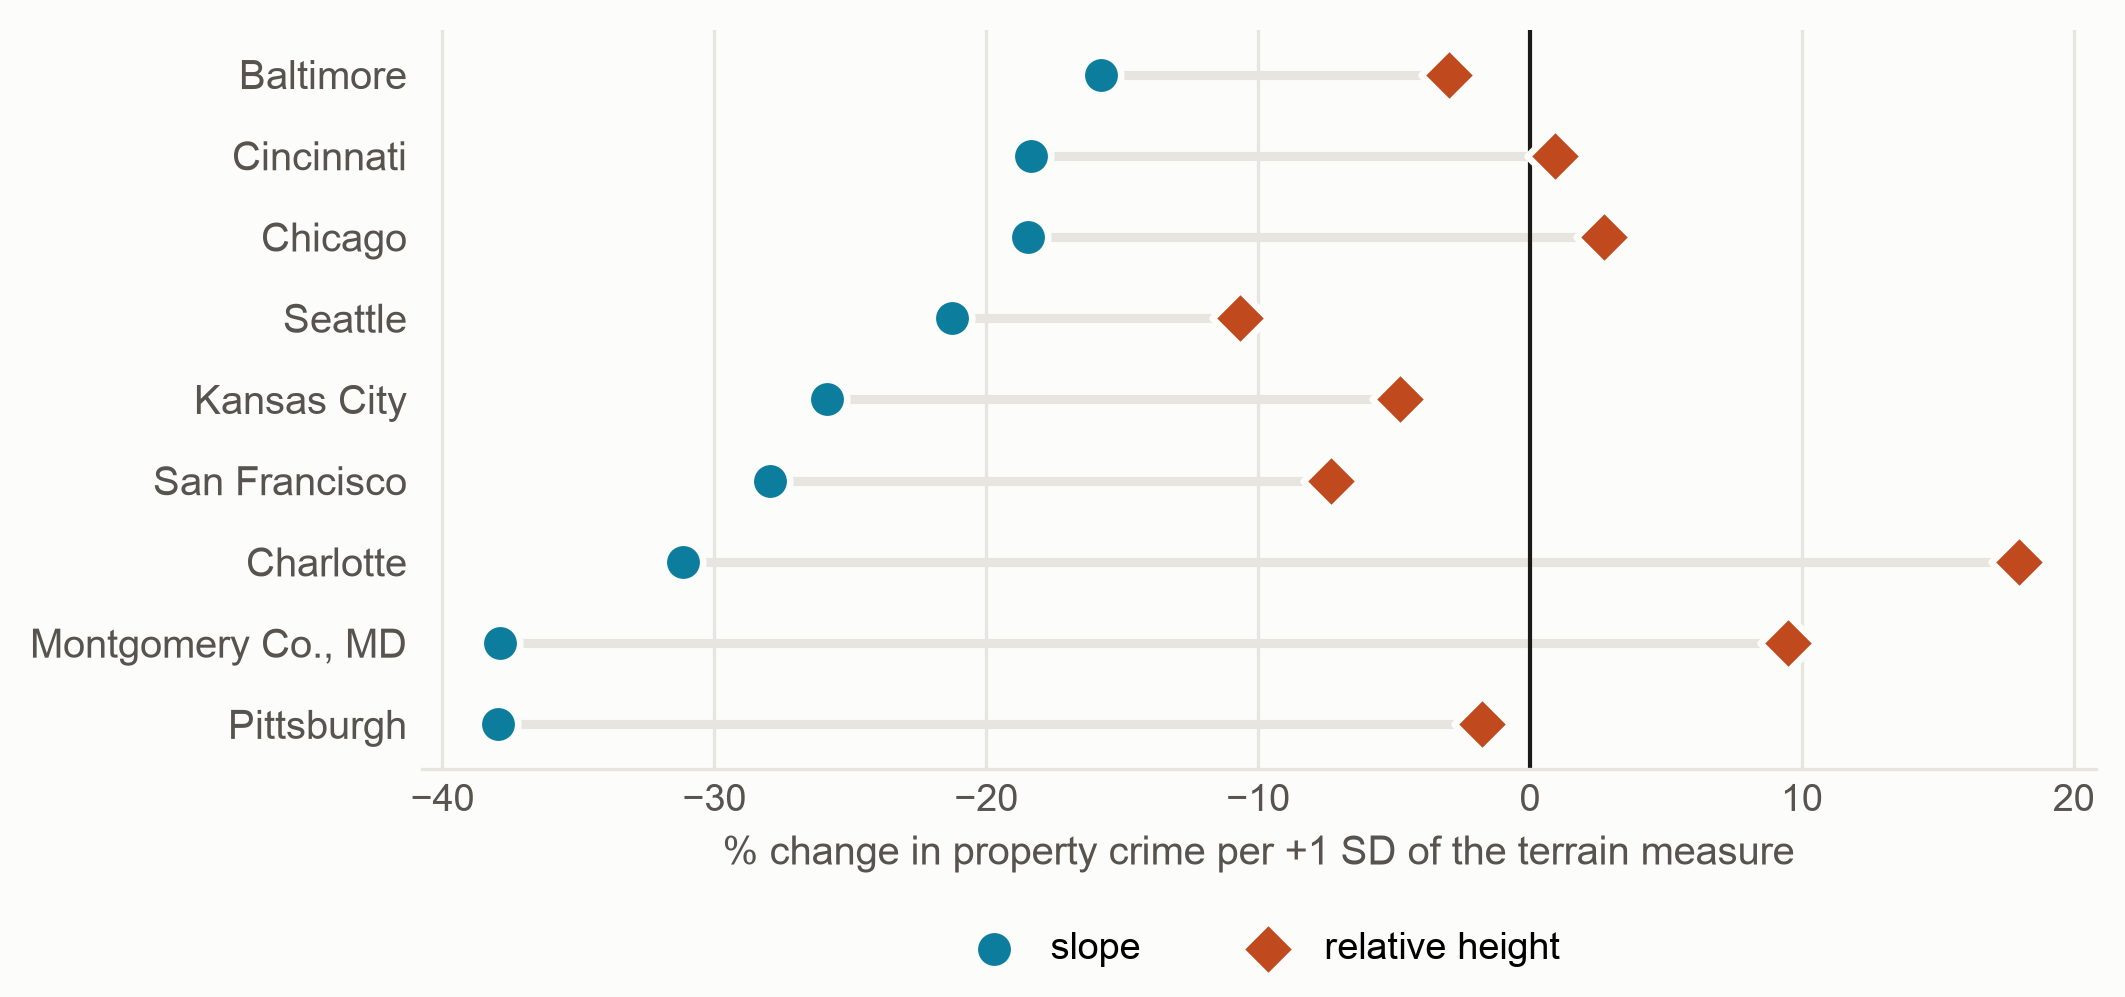
\includegraphics[width=\linewidth]{outputs/fig5_slope_vs_height.png}\fi
\caption{{\bf Slope replicates; relative height does not.} Change in property crime per
one standard deviation of each terrain measure, standardized within city so the two are
on a common scale. Slope is negative in every city. Relative height changes sign, which
is why this paper rests on slope even though the published literature emphasizes
height.}
\label{fig:slopeheight}
\end{figure}

\subsection*{The association is not explained by the cost of carrying loot}

Under a loaded haul account, crimes that remove nothing must show a markedly weaker
slope association than theft, because the loaded return leg is absent. Table~\ref{tab:noloot} and
Fig~\ref{fig:noloot} show that this does not happen.

\begin{table}[!ht]
\centering
\caption{{\bf The no-loot control.} Effect per degree of slope, estimated separately
for theft and for crimes in which nothing is carried away. Differences are bootstrapped
directly over block groups.}
\label{tab:noloot}
\begin{tabular}{lrrrl}
\toprule
City & Theft & Vandalism/arson & Difference & 95\% CI \\
\midrule
Pittsburgh & $-9.79\%$ & $-9.94\%$ & $+0.0017$ & $[-0.017, +0.021]$ \\
San Francisco & $-7.69\%$ & $-7.92\%$ & $+0.0025$ & $[-0.016, +0.020]$ \\
Cincinnati & $-6.38\%$ & $-4.51\%$ & $-0.0198$ & $[-0.040, -0.002]$ \\
Seattle & $-5.61\%$ & $-7.10\%$ & $+0.0160$ & $[+0.005, +0.027]$ \\
\midrule
\textbf{Pooled} & & & $\mathbf{+0.55}$~pp & $\mathbf{[-0.22, +1.32]}$ \\
\bottomrule
\end{tabular}
\end{table}

The pooled difference is $+0.55$ percentage points per degree, with a confidence
interval containing zero. Under the pre-specified decision rule, which required the
two coefficients to be indistinguishable in at least half the cities together with a
pooled interval spanning zero, the loaded haul mechanism is not supported.

\paragraph{A confidence interval containing zero is not evidence of equality.} That
decision rule has a defect I should name rather than leave for a reader to find. A
null result is what an underpowered study also produces, so "the interval contains
zero" is not by itself an argument that the two coefficients are the same. The
question that was actually meant is whether a difference \emph{large enough to
matter} can be ruled out, and that requires an equivalence test and a margin fixed
in advance of looking at the answer.

I set the margin at half the headline effect. The reasoning is that if hauling loot
along a gradient were the mechanism, then removing the load entirely should move the
coefficient by a large fraction of the whole effect, not a sliver of it; half is a
deliberately generous bar for the effort account, since it would pass even if
carrying the goods explained only half of what slope does. On a log scale that is a
margin of $0.0342$, or 3.48 percentage points per degree. Two one-sided tests
against that margin give $p < 10^{-5}$. The theft and no-loot coefficients are
statistically equivalent within half the headline effect. That is a positive
finding about a bounded quantity, not the absence of a finding.

The pattern underneath the pooled figure is what makes this informative rather than
merely underpowered. A loaded haul account requires theft to track slope more
strongly than vandalism in \emph{every} city, because only theft carries the loaded
return leg. It does so in one city out of four. The two individually significant
deviations point in \emph{opposite directions}, with Cincinnati showing the stronger
association for theft and Seattle for vandalism, which is what noise looks like
rather than what a mechanism looks like. And in Pittsburgh and San Francisco, the two
cities with the steepest terrain and therefore the most statistical leverage, the two
coefficients are nearly identical.

\begin{figure}[!ht]
\centering
\ifembedfigs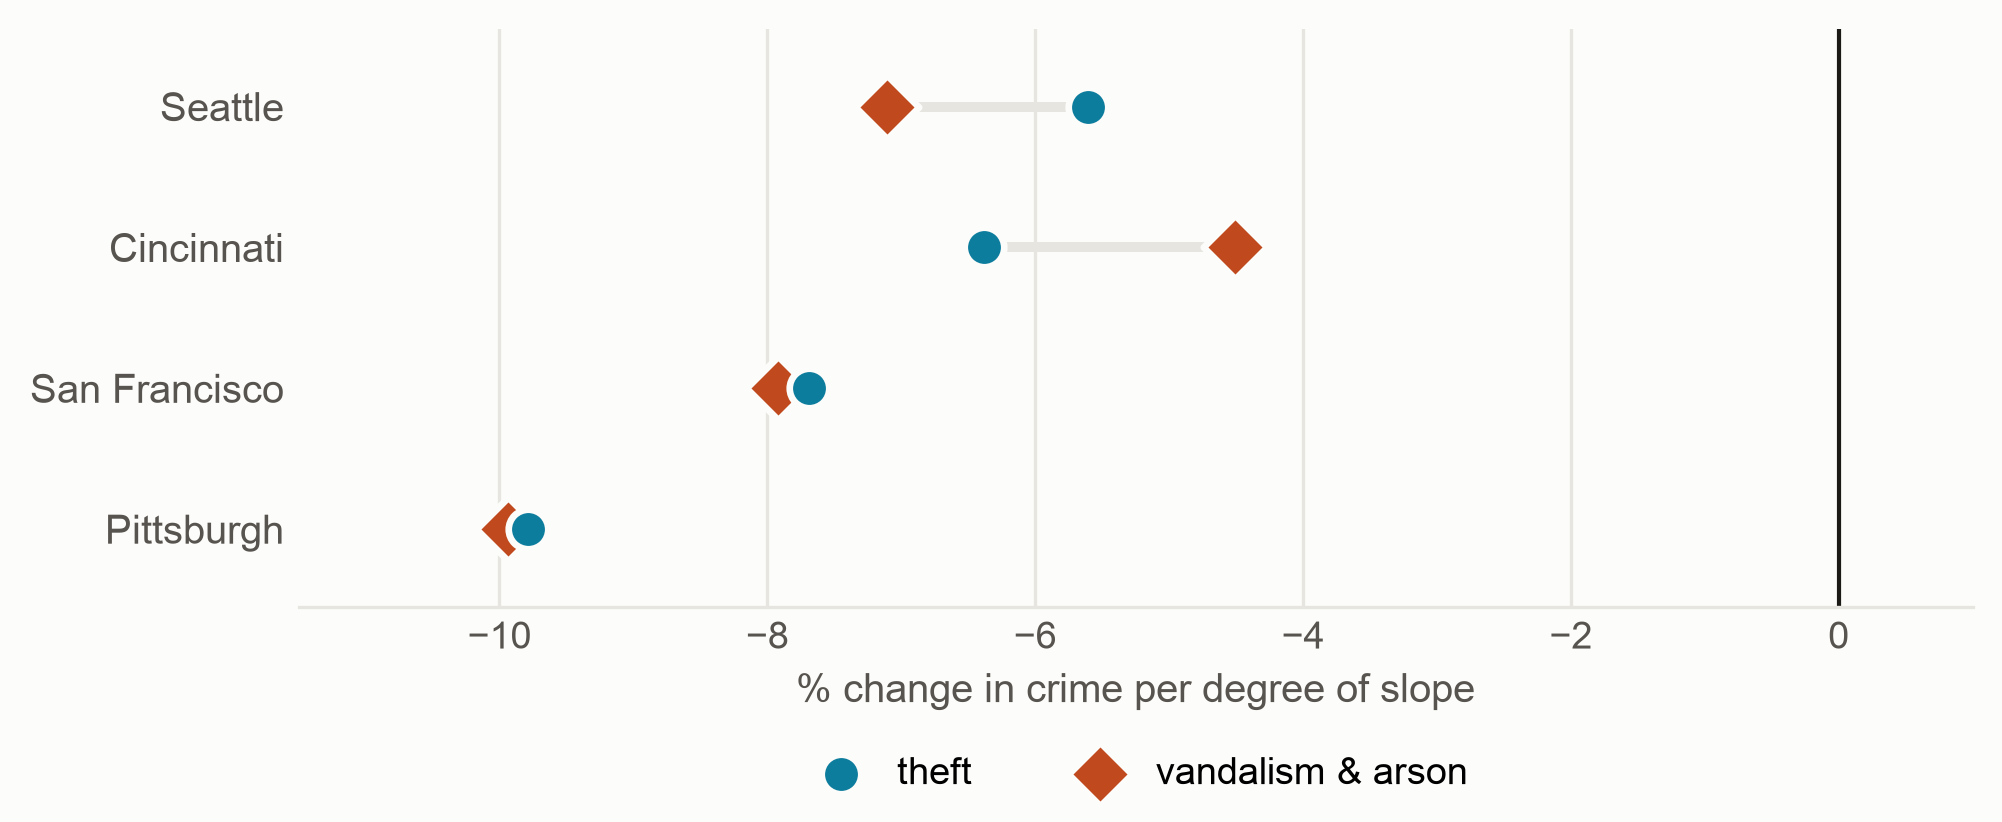
\includegraphics[width=\linewidth]{outputs/fig2_noloot.png}\fi
\caption{{\bf Slope tracks theft and vandalism alike.} Change in crime per
additional degree of street slope, estimated separately for theft, where goods are
carried away, and for vandalism and arson, where nothing is. A loaded haul account requires
the vandalism markers to sit markedly closer to zero, because the loaded return trip is
absent by construction. They do not. In Pittsburgh and San Francisco, the two cities
with the steepest terrain and therefore the most statistical leverage, the two
coefficients nearly coincide. The two cities where a difference is detectable,
Cincinnati and Seattle, differ in \emph{opposite} directions.}
\label{fig:noloot}
\end{figure}

\paragraph{Two objections to the control group, both answered directly.} The
no-loot group is not as homogeneous as calling it "no-loot" implies, and there are
two specific ways that could break the comparison. Both can be tested, because I
re-downloaded the four higher gradient cities keeping the incident timestamp and the
original offense text, which the first pass had discarded.

The first objection is arson. Arson involves preparation, an accelerant, and acute
escape risk, none of which describe breaking a window, so grouping it with vandalism
makes the control less clean. In practice arson is a small part of the group: 1.6\%
of no-loot incidents in Pittsburgh, 2.3\% in Seattle, 3.9\% in San Francisco, and
0.02\% in Cincinnati, where the feed records three arsons in seven years. Dropping
it entirely and re-running the comparison against vandalism alone moves the pooled
difference from $+0.55$ to $+0.09$ percentage points per degree, 95\% CI
$[-2.28, +2.52]$. Estimated on its own where there is enough of it, arson gives
$-4.79\%$ per degree in San Francisco and $-9.30\%$ in Seattle, both squarely inside
the range of everything else.

The second objection is time of day. Vandalism concentrates at night and theft from
vehicles does not, and steep streets are not necessarily equally lit or equally
travelled at three in the morning, so a comparison pooled across all hours confounds
offense type with when the offense happens. I reweighted every no-loot incident so
that the no-loot distribution over the 168 hour-of-day by day-of-week cells matches
theft's, and re-ran the contrast on the reweighted counts. The pooled difference is
$+0.10$ percentage points per degree, 95\% CI $[-2.25, +2.50]$. Both variants pass
the same equivalence test at the same margin ($p < 10^{-5}$).

I did not expect the reweighting to leave the answer this untouched, and I want to
be honest that it is a weaker check than it looks: matching on hour and day does not
match on land use, target type, or micro-location, and a fully matched design is
listed in Further research rather than claimed here.

There is also no gradient with the weight removed (Fig~\ref{fig:ladder}). Vandalism,
which carries nothing, sits in the middle of the ladder. Motor vehicle theft, whose
loot drives itself away and therefore carries no gradient penalty at all, is the least
affected category of any.

\begin{figure}[!ht]
\centering
\ifembedfigs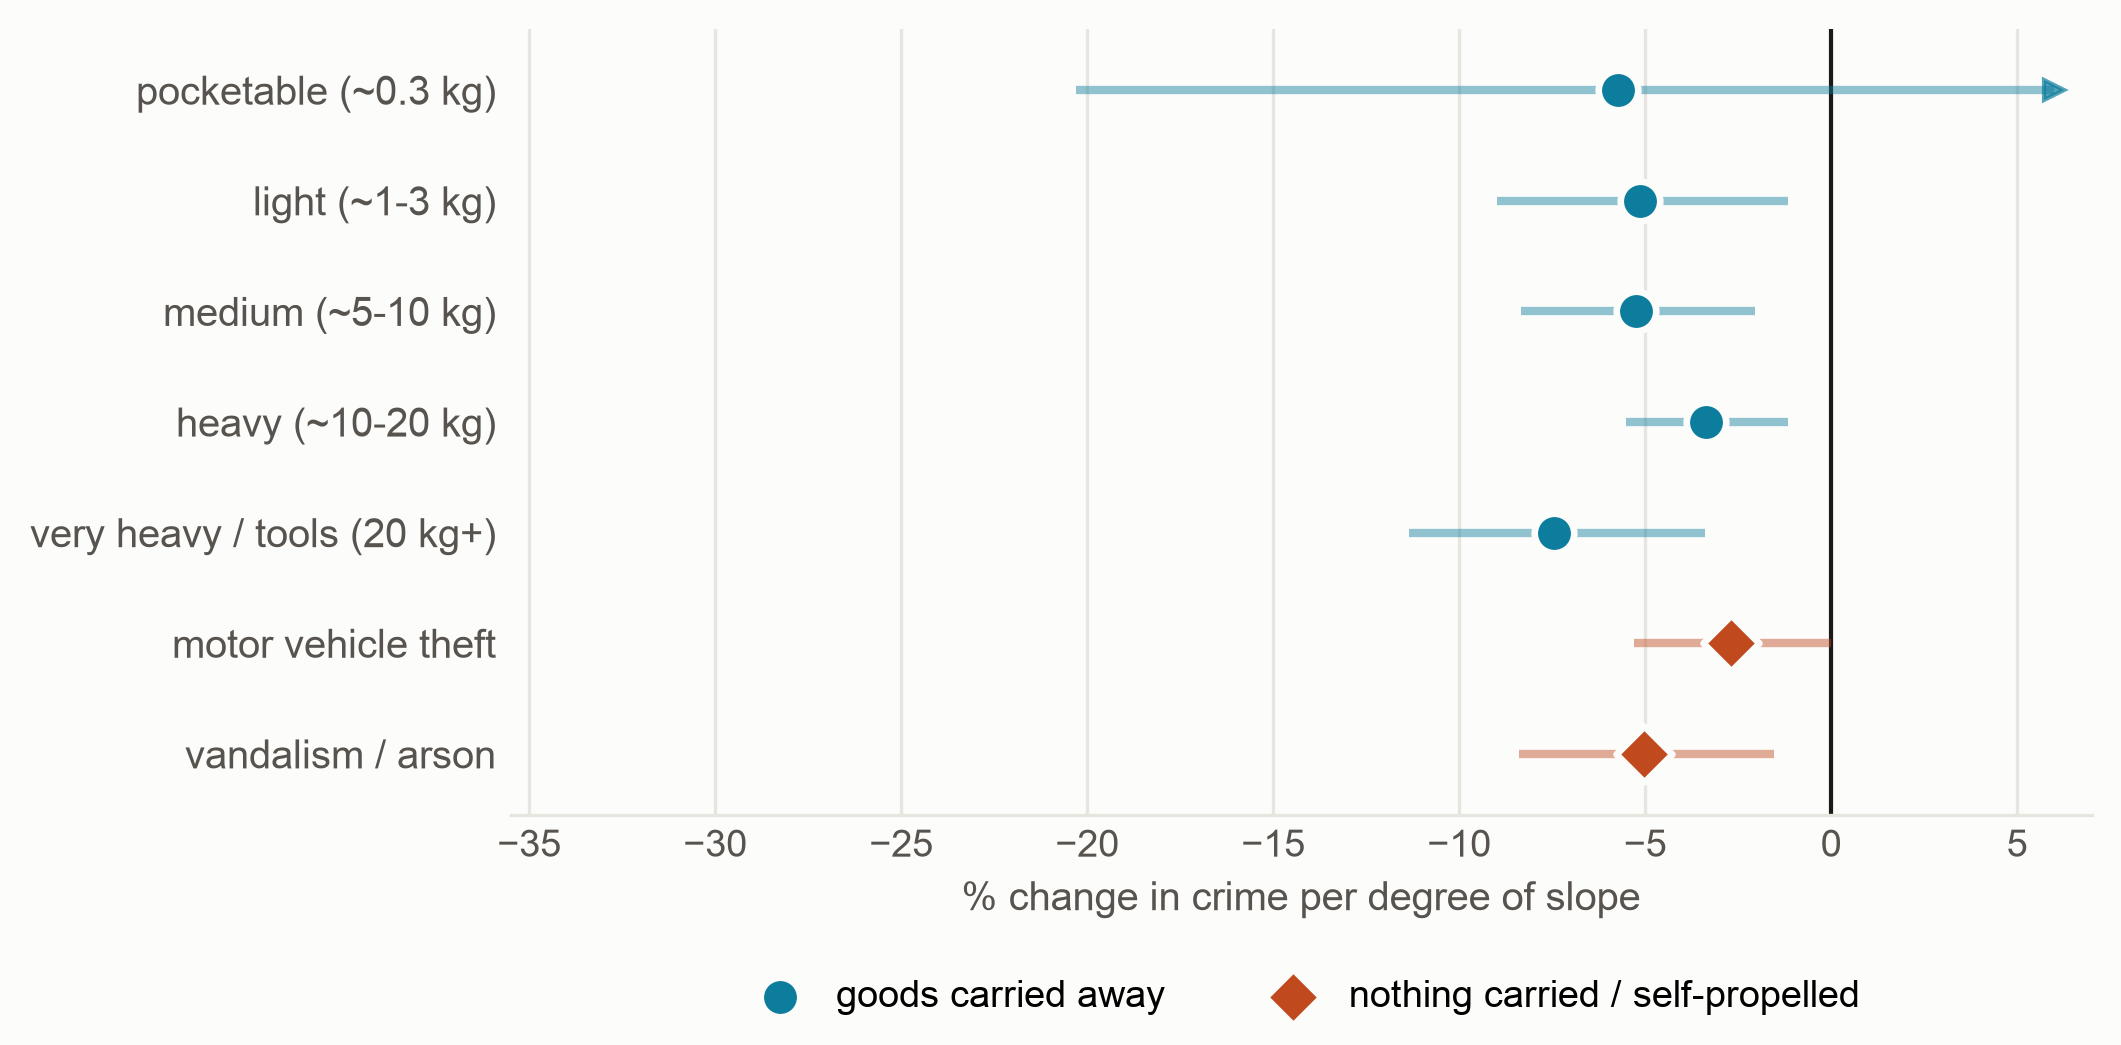
\includegraphics[width=\linewidth]{outputs/fig4_loot_ladder.png}\fi
\caption{{\bf No gradient with the weight carried away.} Change in crime per additional
degree of slope, San Francisco street segments, by how heavy the stolen goods are. Bars
are 95\% confidence intervals; arrowheads mark an interval clipped by the axis. A loaded haul
account requires the association to strengthen down the ladder. It does not. Vandalism and
arson, which carry nothing, sit in the middle of the ordering, and motor vehicle theft,
whose goods drive themselves away, is the least affected category of all.}
\label{fig:ladder}
\end{figure}

\subsection*{A stronger version of the effort theory also fails}

Before abandoning effort I built a better version of it than the one the field uses.
Because metabolic cost is asymmetric in gradient \cite{minetti2002,herzog2014}, a
hilltop is expensive to approach but cheap to leave \emph{carrying goods}, while a
hollow is the reverse. The two legs of the trip therefore price a hill in opposite
directions, and the balance between them is set by how heavy the loot is. That
predicts something the field has never predicted, which is that the terrain
coefficient should rise, and possibly change sign, as goods get heavier.

I built the directional round trip cost surfaces, using Minetti and Herzog metabolic
costs, load scaled, over a ring and spoke quadrature of the catchment, and tested it.
The slope of the coefficient on loot mass is $-0.0018$ per kg, 95\% CI
$[-0.010, +0.018]$. It is not supported.

I also report why this cannot be rescued with more data. Approach cost and loaded
escape cost are both functions of the same gradient field, and they correlate at
$r = -0.80$ with relative height. \emph{Directional movement costs are not
identifiable from an elevation raster.} Separating them would require an asymmetric
network, meaning stairways, one-way access, or walls, and no amount of additional
terrain will do it.

\subsection*{Street network structure absorbs about a quarter of the association}

If steep streets carried less crime by stranding offenders or by carrying fewer passers by,
which are two of the three mechanisms Haberman and Kelsay proposed, then measures of
street network structure should absorb much of the slope coefficient. I test this on
street segments in all four qualifying cities, adding betweenness, intersection
density, permeability, egress count and walk/drive ratio (Table~\ref{tab:mediation}).
Permeability in particular has an established relationship with burglary risk
\cite{johnson2010}, and hills mechanically produce cul-de-sacs and switchbacks, so it
is a plausible mediator rather than merely a control.

\begin{table}[!ht]
\centering
\caption{{\bf Mediation by street network structure.} Effect per degree of slope
before and after adding network measures, San Francisco, Seattle, Cincinnati and
Pittsburgh street segments.}
\label{tab:mediation}
\begin{tabular}{lrrrr}
\toprule
City & Slope effect & + mediators & Attenuation & $n$ segments \\
\midrule
Seattle & $-10.51\%$ & $-9.49\%$ & $+10.2\%$ & 21,087 \\
Pittsburgh & $-6.23\%$ & $-4.27\%$ & $+32.2\%$ & 9,657 \\
San Francisco & $-4.57\%$ & $-5.32\%$ & $-16.8\%$ & 11,185 \\
Cincinnati & $-1.96\%$ & $+1.22\%$ & $+38.6\%$ & 7,787 \\
\midrule
\textbf{Pooled} & $\mathbf{-6.51\%}$ & $\mathbf{-4.96\%}$ & $\mathbf{+24.4\%}$ & \\
\bottomrule
\end{tabular}
\end{table}

Pooled attenuation is 24\%, against a pre-specified threshold of 40\% for supporting
M2. I stated that rule in advance and I report the comparison against it, but I no
longer treat it as a verdict, and the reasons are worth spelling out because they
apply to a common practice.

The first is that coefficient attenuation is not mediation. A formal indirect effect
requires a defined estimand, an assumption of no unmeasured treatment-mediator or
mediator-outcome confounding, an intervention on the mediator one could in principle
perform, and a sensitivity analysis for the violations \cite{imai2010}. None of that
is available here. Slope can shape street layout, but slope and layout are also
jointly produced by development history, engineering constraint and land use, so
conditioning on network structure may be conditioning on a jointly caused variable
rather than isolating a pathway. In a nonlinear model, the change in a coefficient is
not even a clean proportion of anything.

The second is that the 40\% threshold has no theoretical or statistical
justification. I chose it because it felt like a demanding bar. A mechanism that
accounts for a quarter of a large association is substantively important, and calling
it a failure because it fell short of a number I made up would be a mistake. What I
can say is that observable street network structure absorbs roughly a quarter of the
association and does not come close to explaining all of it.

The direction is also inconsistent across cities: San Francisco's coefficient
actually strengthens under the controls, while Cincinnati's large attenuation comes
off a segment level baseline of only $-1.96\%$, small enough that the ratio is
unstable. And betweenness is topological potential, not measured usage; a proper test
of the usage channel needs observed pedestrian and vehicle counts, which I did not
have for any of these cities.

Cincinnati's weak segment level estimate has an identifiable cause rather than being a
substantive finding. Its department jitters incident coordinates, and geocoding error of that kind is a known threat to micro-place work \cite{ratcliffe2004}: 99.9\% of points
are distinct, which gives a median snap distance of 24.6~m against 0.7~m in Seattle
and 2.6~m in Pittsburgh. Against a 107~m median block face, a substantial share of
incidents land on a \emph{neighbouring} segment and 14.6\% miss the 60~m matching
threshold entirely. That is classical attenuation from location error, it is specific
to segment level work, and Cincinnati's grid level estimate of $-5.83\%$ is unaffected.

Two notes on the mediators. First, distance weighted betweenness is confounded with
the treatment. In San Francisco its top ranked streets are residential lanes over the
Twin Peaks ridge, because terrain forces every cross town path through them. I
therefore weight paths by travel time, under which the top ranked streets are the
freeways and arterials, and the two orderings correlate at only $\rho = 0.68$. Second,
a bare earth viewshed proxy turns out to be near collinear with relative height
($r = 0.80$) and cannot be entered as a mediator at all. \textbf{The visibility
mechanism is therefore untested here}, which I state plainly rather than counting it
among the mechanisms I was able to test.

\subsection*{Target availability does not account for it in San Francisco, and the multi-city picture is mixed}

The most serious alternative to a behavioural account is that the effect is
definitional. Steep streets might simply hold fewer parked vehicles, fewer curb cuts
and fewer accessible front doors per unit of measured housing, so they present fewer
targets per unit of nominal exposure. Motor vehicle theft being the least affected
category is consistent with exactly that, since vehicles are the target class a
housing denominator misstates most badly.

The objection does not survive in San Francisco, and it fails before any crime model
is fitted. Regressing target counts on
slope, with the same offset, fixed effects and controls used throughout, shows that
steep San Francisco streets present \emph{more} targets per unit of measured housing
exposure, not fewer: $+2.16\%$ more on-street parking spaces per degree
($[+1.55, +2.77]$), $+1.80\%$ more front doors ($[+0.96, +2.64]$), and $+3.76\%$ more
buildings within 15~m ($[+2.78, +4.74]$). Raw parking density barely varies with
gradient, running 16.3 spaces per 100~m below 1$^\circ$ and 17.6 at 6--12$^\circ$.
What changes is housing density, because hillside blocks are lower density, so the
same length of curb serves fewer dwellings. San Francisco's hills do not lose parked
cars. They lose apartments.

The consequence follows directly (Table~\ref{tab:target}, Fig~\ref{fig:target}).

\begin{table}[!ht]
\centering
\caption{{\bf Replacing the housing denominator with counts of the actual targets at
risk.} San Francisco street segments, effect per degree of slope.}
\label{tab:target}
\begin{tabular}{llrr}
\toprule
Crime & Target denominator & Housing offset & Target offset \\
\midrule
Theft from vehicle & on-street parking spaces & $-6.24\%$ & $-9.66\%$ \\
Motor vehicle theft & on-street parking spaces & $-3.88\%$ & $-6.80\%$ \\
All vehicle crime & on- and off-street parking & $-5.45\%$ & $-8.63\%$ \\
Burglary, all & base addresses & $-3.85\%$ & $-6.32\%$ \\
Residential burglary & base addresses & $-0.97\%$ (n.s.) & $-2.70\%$ \\
Vandalism/arson & parking + front doors & $-6.79\%$ & $-10.90\%$ \\
All property crime & parking + front doors & $-5.93\%$ & $-9.79\%$ \\
\bottomrule
\end{tabular}
\end{table}

\begin{figure}[!ht]
\centering
\ifembedfigs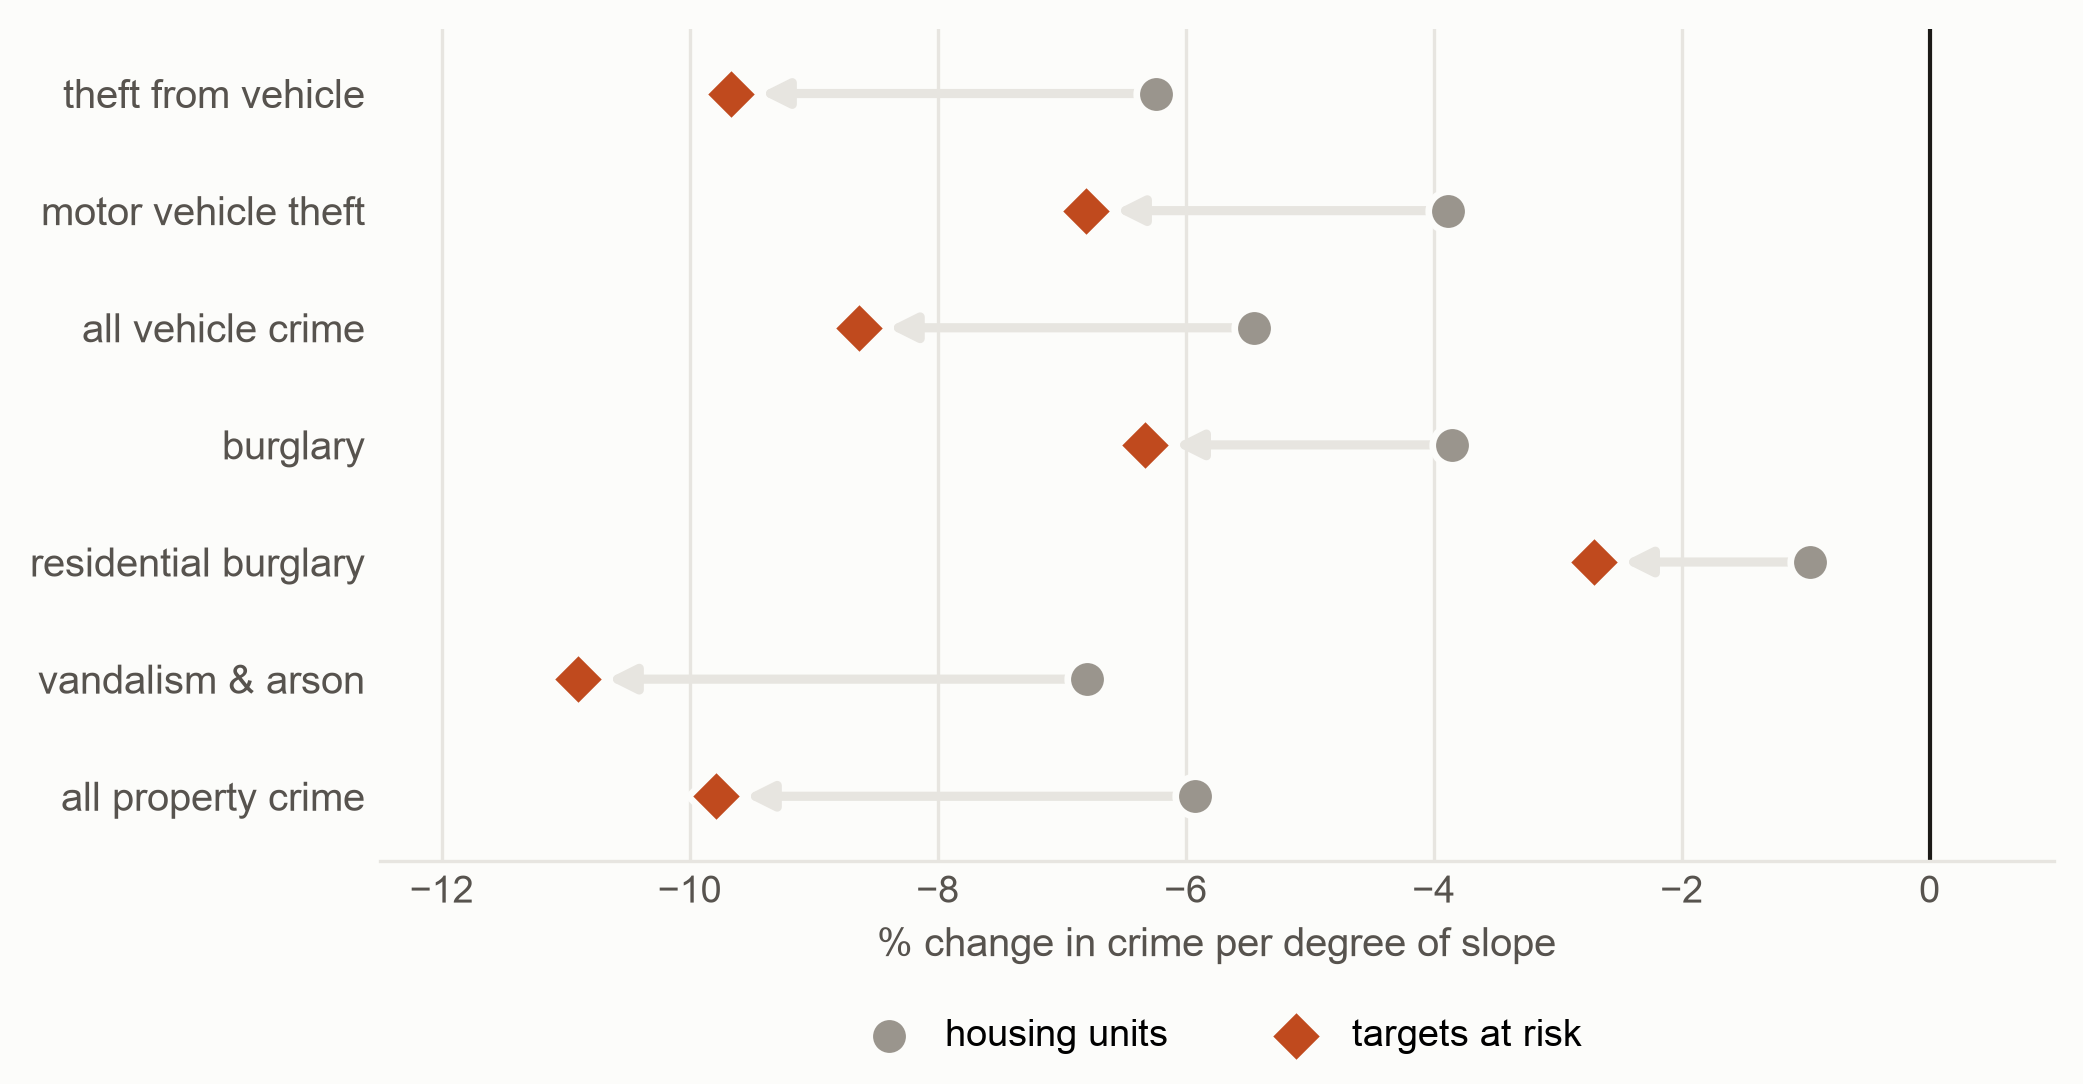
\includegraphics[width=\linewidth]{outputs/fig3_target_denominator.png}\fi
\caption{{\bf Counting the actual targets strengthens the effect rather than
dissolving it.} Each arrow runs from the coefficient estimated on the conventional
housing-unit denominator (grey) to the same coefficient estimated on counts of the
targets genuinely at risk (orange): on-street parking capacity for vehicle crime, front
doors for burglary, and both together for the pooled outcomes. If steep streets simply
held fewer targets per unit of measured housing, counting the targets would drive these
toward zero. Every one moves the other way. Residential burglary, indistinguishable
from zero on the housing denominator, becomes significant once the denominator counts
front doors.}
\label{fig:target}
\end{figure}

The effect does not shrink. It roughly doubles. Shrinkage toward zero is negative in
all forty comparisons, and the result holds when log density is dropped from the
controls, when the sample is restricted to blocks with well measured parking, and when
zero target segments are floored rather than dropped, which matters because those are
exactly the blocks where an artifact would live. Residential burglary, which is
statistically indistinguishable from zero under the housing denominator, becomes
significant once the denominator counts front doors.

In San Francisco, then, target availability does not account for the association. It
was the strongest objection to this paper and it does not survive contact with target
level data there. One implication is worth stating: because target density per housing
unit \emph{rises} with slope in San Francisco, the numbers I report on a housing
denominator are \emph{conservative} estimates of the per-target effect in that city.

The parking data is a real field survey rather than a proxy. San Francisco's on-street
parking census covers 275,339 publicly available spaces across 14,346 blocks and
already excludes driveways, hydrants and bus zones. It matched 89.9\% of segments, and
83.0\% carry non-zero capacity, with \emph{no fallback}, meaning every parking figure
is either measured or absent. Dropped segments are not systematically steeper than
retained ones, at a mean slope of 3.12$^\circ$ against 3.26$^\circ$, so the exclusion
does not select on the treatment. The census was surveyed between 2008 and 2014
against 2018--2026 crime, and space removals since then for bike lanes, parklets and
daylighting cannot be checked against slope, so I flag the direction of that bias as
unknown.

\paragraph{An attempt to extend the target test nationally, which mostly did not
work.} Everything above rests on one city, because the SFMTA parking census and San
Francisco's address point file have no national equivalent. That is too much weight
for one city to carry, so I built the nearest thing that does generalize. Microsoft's
building footprint release covers every city in the panel, and a residential
footprint is a usable stand-in for a front door: a structure someone could enter,
counted directly rather than inferred by spreading a block-group housing total across
cells.

The honest summary is that it did not work well enough to answer the question. A
count of residential footprints per 100~m cell is a small integer, frequently between
one and ten, and using its log as the exposure offset makes the model badly enough
scaled that the inner loop fails to reach its first-order condition. In five of the
nine cities the fit exhausts a two hundred iteration budget with a maximum remaining
score in the hundreds or thousands, and I do not report those estimates
(Table~\ref{tab:targetmulti}).

In the four cities where the model does converge, the denominator barely matters. The
per-degree estimate moves by $+0.99$ percentage points in Baltimore, $-1.49$ in
Kansas City, $-0.57$ in San Francisco and $+0.17$ in Pittsburgh: two toward zero, two
away from it, and all four movements small against a pooled effect of about ten
percent. Pooled across those four, the housing denominator gives $-9.38\%$
$[-14.09, -4.41]$ and the footprint denominator $-9.91\%$ $[-15.69, -3.74]$.

I take three things from this. Nothing here contradicts the San Francisco result.
Nothing here confirms it either, because a footprint count is a much weaker
instrument than an address point file and it is not estimable in most of the panel.
And the San Francisco footprint model in particular runs on 633 cells, since
Microsoft's classifier labels very few San Francisco structures residential, so even
the converged San Francisco figure carries little weight. The target availability
objection is answered in one well-measured city and remains open elsewhere.

\begin{table}[!ht]
\centering
\caption{{\bf Replacing apportioned census housing with a direct count of
residential building footprints.} Same model, same controls, offset only changed.
Cities where the estimator did not reach its first-order condition are reported as
failures rather than as estimates.}
\label{tab:targetmulti}
\begin{tabular}{lrrrr}
\toprule
City & Housing denominator & Footprint denominator & Shift & Cells \\
\midrule
Baltimore & $-7.74\%$ & $-6.74\%$ & $+0.99$ & 1,296 \\
Kansas City & $-13.93\%$ & $-15.41\%$ & $-1.49$ & 17,242 \\
San Francisco & $-7.02\%$ & $-7.59\%$ & $-0.57$ & 633 \\
Pittsburgh & $-9.32\%$ & $-9.14\%$ & $+0.17$ & 14,193 \\
\midrule
\textbf{Random effects pool} & $\mathbf{-9.38\%}$ & $\mathbf{-9.91\%}$ & & \\
\midrule
\multicolumn{5}{l}{\emph{Did not converge, not reported:} Charlotte, Seattle,
Cincinnati, Chicago, Montgomery County MD} \\
\bottomrule
\end{tabular}
\end{table}

\subsection*{Robustness}

\paragraph{Did the estimator actually work?} A Poisson model with several hundred
absorbed fixed effects and a sparse count outcome can fail in ways that leave the
printed coefficient looking entirely ordinary: the maximum likelihood may not exist,
whole fixed effect groups may carry no identifying variation, and the solver may stop
on its iteration cap rather than its tolerance \cite{correia2020}. I did not report
any of this in the first draft. Every city converged on the coefficient tolerance of
$10^{-9}$, in eight to eleven iterations, with a maximum remaining score of
$1.9\times10^{-9}$. There are no separated observations anywhere in the panel and no
singleton block groups. The estimation samples are 40--65\% smaller than the raw cell
tables, the reduction coming from the exposure floor, the geocoding sink filter and
the rule requiring at least three cells per block group. And 1,209 block groups across
the nine cities contain no incidents at all; once their intercepts are absorbed they
contribute nothing to the likelihood, which is the same fact the jurisdiction padding
check below arrives at from the other direction.

\paragraph{Spatial dependence.} Crime clusters and terrain clusters, so cluster robust
standard errors alone might understate uncertainty. Point estimates are stable across
Conley spatial HAC \cite{conley1999} at three bandwidths and eigenvector spatial
filtering: pooled
$-6.18\%$ under cluster robust errors, $-6.25\%$ under Conley HAC at 2~km, and
$-6.13\%$ under the spatial filter. The standard errors do not widen, and the reason
is instructive. Cluster robust standard errors are already 4.7 to 13.7 times larger
than naive independence errors, because census block groups are physically large, with
median diagonals of 500~m in San Francisco, 860~m in Seattle and 1,281~m in
Cincinnati. Clustering on a 1.3~km block group is a \emph{less} restrictive assumption
than a 500~m Conley kernel.

That last comparison is weaker than I made it sound. Cluster robust inference allows
anything inside a block group and assumes independence between them, while a Conley
kernel restricts the form of dependence but lets it cross boundaries, so the two are
not on a scale where one is simply more conservative. Comparing a block group diameter
to a bandwidth does not settle the question. A spatial block bootstrap does: tile the
city into 1~km squares, roughly five block group diameters, resample whole tiles with
replacement and refit, which preserves dependence of any form within a tile including
the kind that crosses block group lines. Doing that in the four higher gradient cities
inflates the standard error by 1.02$\times$ in Pittsburgh, 1.16$\times$ in San
Francisco and 1.30$\times$ in Seattle, and shrinks it slightly in Cincinnati
(0.92$\times$). Seattle's 95\% interval widens from $[-6.96, -4.47]$ to
$[-7.39, -4.00]$. So block group clustering was mildly anticonservative, not
conservative as I claimed, but not by enough to change any conclusion. One further
caveat I flag rather than bury:
residual autocorrelation in Cincinnati is substantial (Moran's $I = +0.338$) and 50
eigenvectors reduce it only to $+0.289$, so Cincinnati's estimate should carry less
weight than its interval implies.

\paragraph{Jurisdiction padding.} Grid cells are clipped to counties, and for
Cincinnati and Pittsburgh a large share of in-county area is suburb that the city
police do not report on, sitting systematically on the uplands above the river
valleys, so the padding is correlated with the treatment. Restricting to block groups
with at least one recorded incident drops 30--40\% of the sample in those two cities
and moves the coefficient by \emph{0.00 percentage points in all four}. A block group
whose counts are uniformly zero contributes nothing to the Poisson likelihood once its
intercept is absorbed, so the fixed effect design is immune to this by construction.

\paragraph{Denominator error.} Replacing area apportionment with building footprint
apportionment cuts Montgomery County's relative height coefficient from $+20.7\%$ to
$+9.5\%$ while barely moving dense San Francisco. Critically, the theft versus no-loot
\emph{contrast} in Montgomery County falls from a gap of $+3.65$ percentage points to
$+0.59$. A measurement error large enough to halve the headline estimate leaves the
contrast intact and in fact makes it more null, which is the central methodological
advantage of an internal comparison.

\paragraph{DEM resolution.} The headline is expressed per degree of slope, and slope is
a derivative whose magnitude depends on the grid it is computed on. The obvious
objection is a units argument. I tested it by fetching a 1~m surface for a matched
San Francisco window and coarsening it to 10~m and 30~m from the same array. The
objection runs the wrong way. Coarsening flattens terrain, from a mean of 6.96$^\circ$
to 5.19$^\circ$, but the flattening is almost purely an \emph{additive offset} rather
than a rescaling, since $\text{slope}_{1\text{m}} = 1.33 + 0.990 \times
\text{slope}_{10\text{m}}$ with $R^2 = 0.992$, and a level shift is absorbed by the
block group fixed effects. Tellingly, the per-standard-deviation column moves
identically to the per-degree column, and the per-SD estimate is unit free by
construction, so units cannot be the explanation. What remains is classical
attenuation: a coarser raster is a noisier proxy for the gradient a person actually
walks, and measurement error in a regressor pulls its coefficient toward zero. Moving
from 10~m to 30~m attenuates the effect by 14\% of itself, and moving to 1~m
strengthens it by 15\%. \textbf{The 10~m estimates reported here therefore understate
the association, and the pooled figure is conservative rather than inflated.}

\paragraph{Contaminated crime class.} The offense text classifier places identity
theft, embezzlement and receiving stolen property on the middle rung of a weight
ladder, because they match the bare word "theft." Possession offenses are worse than
weightless, since the recorded location is where a possessor was stopped rather than
where anything was taken. Dropping that rung entirely moves the pooled estimate from
$-6.61\%$ to $-6.47\%$ on a fixed-effect pool, and lowers heterogeneity from
$I^2 = 0.74$ to $0.66$. Those two figures are on the fixed-effect scale, since the
comparison is like-for-like against the same pool before and after; the point is the
$0.14$ percentage point movement, not the level. The headline does not depend on the
contaminated class.

\paragraph{Classification error, propagated.} The classifier audit found 85.7\%
string level accuracy and 93.7\% incident weighted accuracy, and the analysis then
used the labels as though they were correct. That is a real gap, and it matters most
for the theft against no-loot contrast, which is a comparison between two classifier
outputs. I built $P(\text{true}\mid\text{predicted})$ from the audit, weighted by how
many incidents each string covers, then drew 200 relabellings per city, reassigning
each cell's counts by a multinomial from that matrix, and refit. Label uncertainty
adds a standard deviation of 0.0001 to 0.0007 to the slope coefficient, against
sampling standard errors of 0.0067 to 0.0226. It is 2--3\% of the sampling error and
between 0.02\% and 0.1\% of the total variance, and the pooled estimate and interval
are unchanged to two decimals. Two caveats: the matrix is pooled across cities because
the audit is too small to condition on city, and a string never sampled contributes
nothing, so this is a lower bound on label uncertainty rather than a full accounting.

\paragraph{Observation windows and the pandemic.} The incident windows differ by city
and straddle 2020, so a city effect could partly be a window effect. Splitting at
March 2020 and re-estimating within each period gives $-10.07\%$ before and $-9.72\%$
after in Pittsburgh, $-6.18\%$ and $-5.79\%$ in Seattle, and $-6.22\%$ and $-5.61\%$
in Cincinnati. The association is slightly stronger in the pre-pandemic period in all
three and the differences are well inside each other's intervals. San Francisco cannot
contribute: its feed is capped at the 600,000 most recent incidents, which begin in
February 2021, so there is no pre-pandemic San Francisco window to split. That is a
limitation of my own harvesting rule rather than of the data.

\subsection*{Five measurement findings}

These are byproducts rather than the point of the paper, but each one bears directly
on how this literature should be conducted, and I have not seen any of them stated.

\begin{enumerate}
\item \textbf{Relative height is far less confounded than absolute elevation.} In San
Francisco the correlation with median home value is 0.287 for absolute elevation but
0.047 for the Topographic Position Index, which is roughly a sixfold reduction. What
gets capitalized into land value is the view and the address, not local deviation from
surrounding ground.

\item \textbf{Low relief cities manufacture spurious terrain effects.} Baton Rouge
spans 15.9~m of relief, one standard deviation of relative height is 0.98~m, and the
estimated terrain effect is $+22.9\%$ ($z = 3.1$). A relief floor is a necessary
inclusion criterion and this literature does not have one.

\item \textbf{Results are not robust to the unit of analysis.} In San Francisco,
relative height gives $-9.2\%$ at 100~m cells and $+0.1\%$ at street segments, while
slope is negative under both. Since the published studies use different units, this is
a live threat to their comparability.

\item \textbf{Per-degree slope coefficients are not comparable across studies using
different elevation resolutions,} and this literature does not currently report DEM
resolution as a matter of course. Mine are computed on 10~m data and would be roughly
15\% stronger on 1~m data.

\item \textbf{Offense text classifiers silently destroy classes and must be
validated.} I validated mine against 511 hand coded description strings drawn from all
31 registry cities, using a holdout sample drawn after the revision was written so
that the improvement could be measured honestly. Accuracy is 85.7\% string level and
93.7\% incident weighted on the holdout, and the control class is clean, with NO\_LOOT
precision 0.956 and recall 1.000. But the audit found four defects that had been
completely silent, in that totals looked plausible, models converged and coefficients
were stable. NIBRS 23G and 24I, which are theft of motor vehicle parts and of license
plates, were being counted as motor vehicle theft, which in Seattle merged 32,501
parts thefts into 50,824 real vehicle thefts and left the heaviest loot rung empty.
Ohio charges vandalism as "CRIMINAL DAMAGING/ENDANGERING," which a pattern written for
"criminal damage" does not match, so Cincinnati's 28,513 no-loot records fell to an
unclassified bucket and the city was excluded from this paper's primary test for
apparently lacking vandalism data. Los Angeles publishes vehicle theft as
"VEHICLE - STOLEN," which contains no "stolen vehicle" in that order. And
\texttt{Series.astype(str)} preserves NaN on pandas 3.0.5, so a single null
description column turned an entire concatenated string into NaN. Cross-city crime
research that maps free text offense descriptions onto analysis categories should
report a hand coded validation sample as a matter of course, and I know of none that
does.
\end{enumerate}

% ---------------------------------------------------------------------------
\section*{Discussion}

Haberman and Kelsay closed their paper by naming three reasons steep blocks might
carry less crime: physical cost, difficulty of escape, and lower usage. I set out to
test all three on property crime across nine cities and added a fourth of my own.
None of them accounts for what I find, but the four results are of very different
strengths and I want to be exact about which is which, because an earlier draft of
this paper treated them as interchangeable and they are not.

I should also note a bookkeeping problem with my own framing. Haberman and Kelsay
named escape difficulty and lower usage as two mechanisms; I collapsed them into one
network and exposure test, introduced affluence as a third of my own, and later added
target availability as a fourth. So this is not one clean test for each of their
three. Actual pedestrian and vehicle usage, and visibility, remain unmeasured
throughout.

\textbf{The loaded haul account is the one genuinely bounded result.} Crimes in which
nothing is carried away show the same association with slope as theft, and an
equivalence test rules out a difference larger than half the headline effect. That
survives dropping arson and matching the two offense groups on hour and day of week.
There is no gradient across loot mass, and motor vehicle theft, whose goods drive
themselves away, is the \emph{least} affected category. A directional round trip
model, which prices the loaded return leg explicitly, fares no better. What this
rules out is a specific quantitative claim: that the association is driven mainly by
the metabolic cost of moving stolen property along a gradient. It does not rule out
the cost of \emph{approaching} a target, the offender's perception of that cost,
search costs, or escape risk. Those remain live and I have not tested them.

\textbf{Escape difficulty and lower usage are partly supported.} Betweenness,
intersection density, permeability, egress count and walk/drive ratio absorb about a
quarter of the slope coefficient pooled across four cities. That fell short of a 40\%
threshold I had written down in advance, but I no longer treat that as a verdict: the
number was arbitrary, coefficient attenuation is not a causal indirect effect
\cite{imai2010}, and a mechanism accounting for a quarter of a large association is
substantively important. This is the least rejected of the candidate mechanisms and
the one I would bet on. Two things keep it untested rather than confirmed: every
measure I have describes the street's topology rather than who actually uses it, and
the visibility channel could not be entered at all, because a bare earth viewshed
proxy is near collinear with terrain itself.

\textbf{Affluence is controlled between block groups, not eliminated.} An earlier
draft said it "fails by construction." That was wrong, and it is worth explaining
why, because the error is easy to make. Income, home value, tenure and vacancy are
measured at block group level, so the fixed effects absorb them rather than the
covariates controlling them separately; the covariates are doing very little work. And
within a single block group, household wealth, home security, private surveillance,
housing type and willingness to report can all still covary with slope. Given that Ye
and Becker document exactly this sorting on the vertical dimension of American cities
\cite{yebecker2018}, within-block-group affluence gradients are a live concern rather
than a hypothetical one. What I can say is that the association is not driven by
between-neighbourhood sorting. That is a real result and it is less than ruling
affluence out.

\textbf{Target availability does not account for it in San Francisco; elsewhere it is
mixed.} If steep streets simply held fewer parked cars and front doors per unit of
measured housing, counting the targets directly should have collapsed the effect. In
San Francisco, with a field-surveyed parking census and an address point file, it
roughly doubles instead. My attempt to extend the test nationally on building
footprint counts is largely uninformative: it fails to converge in five of nine
cities, and where it does converge the denominator moves the estimate by less than
1.5 percentage points either way. I would summarize this as: the objection is dead in
the one city where the target data is good enough to kill it, and unresolved
everywhere else.

That leaves an association which is large, consistent in sign across nine cities, and
robust to the unit of analysis, to spatial dependence under a block bootstrap, to
label uncertainty in the classifier, to the observation window, to several denominator
specifications, and to dropping the one crime class with meaningful contamination, and
which is not accounted for by any mechanism I have been able to test.

The honest position is to report that rather than to supply a fifth story. Two
directions seem worth pursuing, and I can rule out neither:

\emph{Exposure to offenders rather than to targets.} Every mediator I tested describes
the \emph{street}. None of them measures who actually walks or drives along it.
Foot traffic data would test whether steep streets are simply encountered less often,
which is a version of "lower usage" that betweenness, being a topological rather than
a behavioural quantity, may fail to capture.

\emph{Perceived rather than actual cost.} My tests reject \emph{metabolic}
accounting. They do not reject the possibility that gradient reads as effort, or
remoteness, or conspicuousness at the moment a target is selected, independent of what
climbing actually costs. That would explain why the association does not scale with loot
mass while still being about the offender's decision. Distinguishing it requires
offender level data, not more terrain.

\emph{Offender location choice.} The design that would actually settle this is not
another aggregate model. It is a discrete choice model over the places an offender
could have gone and did not, using cleared offenses with a known origin. That
literature exists and is well developed: Frith, Johnson and Fry separate travel effort
from familiarity and from local versus non-local guardianship at street segment
resolution \cite{frith2017}; Johnson and Summers show road network accessibility
shaping adult offenders' choices for theft from vehicles \cite{johnsonsummers2015};
Clare and colleagues show physical barriers and connectors altering burglars'
selections \cite{clare2009}. None of it is available from municipal open data, which
publishes incidents rather than offenders. That is the boundary of this design, not a
gap in the field.

I want to be careful about practical implications, because this is the point at which
an unidentified association is most likely to be misused. I have shown a conditional
association and ruled out one specific mechanism for it. I have not shown that
gradient deters offenders, and it would be wrong to read this paper as saying hillside
neighbourhoods are intrinsically safer or that access is a policy lever. Reported
crime is not victimization, reporting rises with income, and income rises with
elevation, so part of what these coefficients describe could be who calls the police
rather than who offends.

\subsection*{Limitations}

This study uses reported crime only, and reporting rates rise with income, which
correlates with elevation. Crime type harmonization across departments is coarse where
cities publish only a top level offense category, and in the NIBRS cities in
particular the top two rungs of the loot ladder cannot be distinguished at all, which
compresses the ladder and biases any mass gradient toward zero. That is why I rest the
mechanism argument on the no-loot control rather than on the ladder. Bare earth
elevation models still contain built terrain. I have no offender residence data, so
crime location choice models are out of reach.

Six limitations deserve particular emphasis.

\textbf{This is an observational design and it does not identify deterrence.} Block
group fixed effects remove between-neighbourhood differences and nothing else. Slope
is not randomly assigned within a block group, and a steep street and a flat one in
the same block group can differ in density, housing form, commercial use, lighting,
frontage, parking regulation, transit access, road width and reporting behaviour. Any
of those could produce the association without gradient doing anything.

\textbf{The slope variable was selected after seeing data}, since the analysis plan
specifies relative height, so the headline is a discovery rather than a confirmatory
test; Pittsburgh, Baltimore and Charlotte provide partial out of sample support but
were analyzed knowing what I was looking for.

\textbf{Between-city heterogeneity is severe.} $I^2 = 0.75$ among the higher gradient
cities, with a Q-profile interval from 0.19 to 0.98, and the prediction interval for
a new city includes zero. The moderator model accounts for 59\% of the between-city
variance; the remaining 41\% is unexplained.

\textbf{The visibility and usage mechanisms were never tested.} A bare earth viewshed
proxy cannot be separated from terrain, and I have no observed pedestrian or vehicle
counts for any city, so the most plausible surviving mechanism is the one I have the
least evidence about.

\textbf{The target denominator result rests on one city.} San Francisco has a
field-surveyed parking census and an address point file. The nine-city extension uses
building footprints, which are a much cruder stand-in for a front door, and it gives a
split result.

\textbf{The mechanism remains unidentified}, and I do not offer one I cannot test.

The exploratory phase of this project ran many specifications. The tests reported as
confirmatory were fixed in a written analysis plan before the confirmatory dataset
existed, all deviations from it are itemized in that document's addendum, and
everything else is labelled exploratory. I want to be precise about the status of that
plan: it was written down and timestamped locally, but it was not deposited in a
public registry before the analysis ran. It is therefore a \emph{pre-specified
analysis plan}, not a pre-registration, and I do not claim the latter.

% ---------------------------------------------------------------------------
\section*{Conclusion}

Steeper streets carry less recorded property crime, in every one of the nine American
cities I looked at, and among the four with the most measurable gradient the pooled
estimate is about seven percent per degree, with a prediction interval for a new city
that runs from thirteen percent down to nothing at all. That much replicates a finding
already established for robbery in a single city and extends it to property crime
across many, while showing that the magnitude does not transport.

What does not follow is the explanation. The association is not driven by the cost of
carrying loot: crimes in which nothing is removed track slope just as closely as
crimes in which something is, and an equivalence test rules out a difference larger
than half the headline effect. It is not mainly street layout, which absorbs about a
quarter of it. It is not between-neighbourhood affluence, though within-neighbourhood
affluence remains a live possibility I cannot exclude. And in the one city where I can
count the actual targets at risk, it is not target scarcity, since hillside blocks
carry more parked cars and more front doors per household than flat ones do.

So: a large, consistent, well measured association between street gradient and
recorded property crime, whose mechanism I cannot identify after four attempts. I
would rather end a paper there than invent a reason. The design that could settle it
is a choice model over the places offenders passed up, and that needs data municipal
portals do not publish.

% ---------------------------------------------------------------------------
\section*{Ethics and responsible use}

The data are public, which is not the same as unproblematic. Every source used here
is published by a government agency for general use, no record was obtained under a
restricted-use agreement, and no human subjects research approval was required. But
incident level coordinates, dates and offense descriptions can identify sensitive
locations and stigmatize small places, and at least one department in this panel
already treats that as a live concern: Cincinnati jitters its coordinates, which is a
deliberate privacy measure that also degrades segment level analysis, as reported
above.

Three choices follow from that. Nothing below the 100~m grid cell or the street
segment is reported anywhere in this paper, and no map in it resolves an individual
incident. Where a replication archive is released it will distribute retrieval scripts
and the aggregated analytic units rather than republishing raw point records, since
the portals are the appropriate publisher of their own data and their terms and
redaction practices can change after I have downloaded a copy.

The interpretive risk deserves saying plainly, because it is larger than the
disclosure risk. A result of the form "hills have less crime" is exactly the kind of
finding that gets absorbed into real estate marketing, insurance pricing, patrol
allocation or neighbourhood risk scoring, and it would be absorbed with none of the
qualifications in this paper attached. I want to state the two that matter most.
First, this is reported crime, and reporting rises with income, which rises with
elevation \cite{yebecker2018}; a lower count is not demonstrably less victimization.
Second, the mechanism is unknown, so nothing here supports acting on gradient as a
cause. A paper that cannot say why an association exists is not a basis for allocating
enforcement or pricing risk, and I would rather say so than leave it to inference.

% ---------------------------------------------------------------------------
\section*{Software, automation and AI tooling}

Because the classifier and several derived variables drive the central claims, and
because it is now a reasonable thing for a reader to want to know, I state exactly
what produced what.

\textbf{The offense classifier is deterministic and rule based.} It is an ordered
cascade of regular expressions over the concatenated offense description fields, with
a fixed loot mass ladder attached to its classes. It is not a machine learning model
and it is not a language model; it does not learn from the data it labels, and the
same string always receives the same class. The complete rule set is released with the
code, along with the 511 hand-coded strings, the confusion matrices and the failure
patterns. The hand coding was done by me.

\textbf{The derived exposure variables are deterministic geometry.} Building footprint
apportionment, on-street parking apportionment, front door counts, street network
measures and every terrain surface are computed by published algorithms over public
inputs, with no inference step and no model fitting.

\textbf{Generative AI was used in preparing this work, and here is where.} I used
Anthropic's Claude as a coding assistant throughout the analysis pipeline and as a
drafting and editing assistant for the manuscript. Concretely, it wrote and revised
substantial parts of the Python that harvests the data, computes the terrain
measures, fits the models and draws the figures; it helped draft and revise prose;
and it was used to check arguments and to search for objections. It was not used to
label any incident, to select any specification on the basis of results, or to
generate any number reported in this paper: every figure in every table comes from
code executing over the data. Several errors described in this paper and its
supplement were found through that process, and several were introduced by it; the
classifier defects listed in the measurement findings are of the latter kind. All
analytic decisions, the hand coding, and the final content are mine, and I take
responsibility for them.

No records were transmitted to a third-party service for labelling or inference. The
data all came from public government endpoints, and every model fit ran locally.

% ---------------------------------------------------------------------------

\subsection*{Further research}

There are several directions this work could go. Namely, foot traffic data would
directly test the "lower usage" channel that betweenness only approximates, and
commercial datasets for this now exist at street segment resolution. Further, a
natural experiment is available and nobody has used it: Pittsburgh maintains over 700
public staircases, individually inventoried, with documented closures and repairs.
A staircase collapses the walking cost of a slope while doing nothing at all to the
driving cost, the view, or the property value, which makes a closure about as clean a
shock to pedestrian access as terrain research is ever likely to get. The same design
exists at larger scale in Medellín, where the Metrocable gondolas and the Comuna 13
outdoor escalators cut the effort cost of steep hillside neighbourhoods on known dates,
and where the wealth gradient runs the opposite way to the American cities studied
here.

Finally, this paper treats terrain as a property of places. A version that treated it
as a property of \emph{trips} would be better, but it requires offender origin data
that is not public.

\section*{Supporting information}

\paragraph*{S1 Appendix.} {\bf Analysis plan and deviations.} Hypotheses, inclusion
rules and decision criteria fixed before the confirmatory dataset existed, with nine
itemized deviations.

\paragraph*{S2 Appendix.} {\bf Reporting checklist and table index.} STROBE checklist,
an index of all thirty-two result tables, and the full specification history including
the four abandoned analysis phases.

\paragraph*{S3 Data.} {\bf Classifier validation.} 511 hand coded offense description
strings with confusion matrices, per class precision and recall, and documented
failure patterns.

\section*{Acknowledgments}

All of the data used here is public: elevation from the USGS 3D Elevation Program,
crime from municipal open data portals, demographics and geography from the US Census
Bureau, street networks from OpenStreetMap, and building footprints from Microsoft.
None of it required an API key, which means the entire pipeline can be reproduced by
anyone without credentials, and I think that matters more than it usually gets credit
for.

I would like to thank the open data staff at the nine city governments whose portals
made this possible. Work like this is completely dependent on people who publish
incident level data with coordinates and then keep publishing it.

% ---------------------------------------------------------------------------
% For submission, switch to: \bibliographystyle{plos2015} \bibliography{references}
\begin{thebibliography}{10}

\bibitem{haberman2021}
Haberman CP, Kelsay JD.
\newblock The topography of robbery: does slope matter?
\newblock J Quant Criminol. 2021;37(3):625--645.

\bibitem{breetzke2012}
Breetzke GD.
\newblock The effect of altitude and slope on the spatial patterning of burglary.
\newblock Appl Geogr. 2012;34:66--75.

\bibitem{kimwo2023}
Kim YA, Wo JC.
\newblock Topography and crime in place: the effects of elevation, slope, and
betweenness in San Francisco street segments.
\newblock J Urban Aff. 2023;45(6):1120--1144.

\bibitem{bikesf2026}
Christiansen E, Pires SF.
\newblock Topography, accessibility, and the built environment: explaining spatial
patterns of bicycle theft.
\newblock Int J Sustain Transp. 2026.
\newblock doi:10.1080/15568318.2026.2659601

\bibitem{biketoronto2026}
Christiansen E.
\newblock Exploring bicycle theft through topography, street centrality, and the
built environment: a spatial analysis of Toronto, Canada.
\newblock Comput Urban Sci. 2026;6(11).
\newblock doi:10.1007/s43762-025-00232-7

\bibitem{weiss2001}
Weiss AD.
\newblock Topographic position and landforms analysis.
\newblock In: ESRI User Conference; 2001.

\bibitem{minetti2002}
Minetti AE, Moia C, Roi GS, Susta D, Ferretti G.
\newblock Energy cost of walking and running at extreme uphill and downhill slopes.
\newblock J Appl Physiol. 2002;93(3):1039--1046.

\bibitem{herzog2014}
Herzog I.
\newblock Least-cost paths: some methodological issues.
\newblock Internet Archaeol. 2014;36.
\newblock doi:10.11141/ia.36.5

\bibitem{brantingham1993}
Brantingham PL, Brantingham PJ.
\newblock Environment, routine, and situation: toward a pattern theory of crime.
\newblock In: Routine Activity and Rational Choice. Transaction; 1993. p. 259--294.

\bibitem{johnson2010}
Johnson SD, Bowers KJ.
\newblock Permeability and burglary risk: are cul-de-sacs safer?
\newblock J Quant Criminol. 2010;26(1):89--111.

\bibitem{weisburd2015}
Weisburd D.
\newblock The law of crime concentration and the criminology of place.
\newblock Criminology. 2015;53(2):133--157.

\bibitem{cohen1979}
Cohen LE, Felson M.
\newblock Social change and crime rate trends: a routine activity approach.
\newblock Am Sociol Rev. 1979;44(4):588--608.

\bibitem{conley1999}
Conley TG.
\newblock GMM estimation with cross sectional dependence.
\newblock J Econom. 1999;92(1):1--45.

\bibitem{yebecker2018}
Ye V, Becker C.
\newblock The Z-axis: elevation gradient effects in urban America.
\newblock Reg Sci Urban Econ. 2018;70:312--329.
\newblock doi:10.1016/j.regsciurbeco.2017.10.002

\bibitem{yebecker2024}
Ye V, Becker C.
\newblock Moving mountains: geography, neighborhood sorting, and spatial income
segregation.
\newblock Working paper; 2024.

\bibitem{frith2017}
Frith MJ, Johnson SD, Fry HM.
\newblock Role of the street network in burglars' spatial decision-making.
\newblock Criminology. 2017;55(2):344--376.
\newblock doi:10.1111/1745-9125.12133

\bibitem{johnsonsummers2015}
Johnson SD, Summers L.
\newblock Testing ecological theories of offender spatial decision making using a
discrete choice model.
\newblock Crime Delinq. 2015;61(3):454--480.
\newblock doi:10.1177/0011128714540276

\bibitem{clare2009}
Clare J, Fernandez J, Morgan F.
\newblock Formal evaluation of the impact of barriers and connectors on residential
burglars' macro-level offending location choices.
\newblock Aust N Z J Criminol. 2009;42(2):139--158.
\newblock doi:10.1375/acri.42.2.139

\bibitem{horn1981}
Horn BKP.
\newblock Hill shading and the reflectance map.
\newblock Proc IEEE. 1981;69(1):14--47.

\bibitem{silva2006}
Santos Silva JMC, Tenreyro S.
\newblock The log of gravity.
\newblock Rev Econ Stat. 2006;88(4):641--658.
\newblock doi:10.1162/rest.88.4.641

\bibitem{correia2020}
Correia S, Guimar\~aes P, Zylkin T.
\newblock Fast Poisson estimation with high-dimensional fixed effects.
\newblock Stata J. 2020;20(1):95--115.
\newblock doi:10.1177/1536867X20909691

\bibitem{imai2010}
Imai K, Keele L, Tingley D.
\newblock A general approach to causal mediation analysis.
\newblock Psychol Methods. 2010;15(4):309--334.
\newblock doi:10.1037/a0020761

\bibitem{higgins2002}
Higgins JPT, Thompson SG.
\newblock Quantifying heterogeneity in a meta-analysis.
\newblock Stat Med. 2002;21(11):1539--1558.
\newblock doi:10.1002/sim.1186

\bibitem{viechtbauer2007}
Viechtbauer W.
\newblock Confidence intervals for the amount of heterogeneity in meta-analysis.
\newblock Stat Med. 2007;26(1):37--52.
\newblock doi:10.1002/sim.2514

\bibitem{intHout2014}
IntHout J, Ioannidis JPA, Borm GF.
\newblock The Hartung-Knapp-Sidik-Jonkman method for random effects meta-analysis is
straightforward and considerably outperforms the standard DerSimonian-Laird method.
\newblock BMC Med Res Methodol. 2014;14:25.
\newblock doi:10.1186/1471-2288-14-25

\bibitem{ratcliffe2004}
Ratcliffe JH.
\newblock Geocoding crime and a first estimate of a minimum acceptable hit rate.
\newblock Int J Geogr Inf Sci. 2004;18(1):61--72.
\newblock doi:10.1080/13658810310001596076

\end{thebibliography}

\end{document}
